%% ----------------------------------------------------------------
%% Thesis.tex
%% ---------------------------------------------------------------- 
\documentclass{ecsthesis}      % Use the Thesis Style
\graphicspath{{../figures/}}   % Location of your graphics files
\usepackage{natbib}            % Use Natbib style for the refs.
\hypersetup{colorlinks=true}   % Set to false for black/white printing
%% ----------------------------------------------------------------
%% Definitions.tex
%% ---------------------------------------------------------------- 
\newcommand{\BibTeX}{{\rm B\kern-.05em{\sc i\kern-.025em b}\kern-.08em T\kern-.1667em\lower.7ex\hbox{E}\kern-.125emX}}

%% People
\newcounter{address}
\setcounter{address}{1}
\renewcommand{\theaddress}{\textsuperscript{\fnsymbol{address}}}
\newcommand{\address}[1]{\refstepcounter{address}\theaddress#1\\}
\newcommand{\Name}[3]{\texorpdfstring{\href{mailto:#3}{#2}#1}{#2}\xspace}
\newcommand{\Tsagkopoulos}[1]{\Name{#1}{Nikolaos Chrysovalantis Tsagkopoulos}{n.tsagko@gmail.com}}

%% Dingbats
\newcommand{\tick}{\ding{51}}
\newcommand{\cross}{\ding{55}}

%% Calculus
\newcommand{\pd}[2]{\ensuremath{\frac{\partial #1}{\partial #2}}\xspace}
\newcommand{\fd}[2]{\ensuremath{\frac{d #1}{d #2}}\xspace}
\newcommand{\dint}{\ensuremath{\int\!\!\!\int}\xspace}
\newcommand{\tint}{\ensuremath{\int\!\!\!\int\!\!\!\int}\xspace}

%% Math Sets
\newcommand{\Q}[1]{\ensuremath{\mathbb{#1}}\xspace}
\newcommand{\R}{\Q{R}}

%% Matrix, Vector
\newcommand{\V}[1]{\ensuremath{\boldsymbol{#1}}\xspace}
\newcommand{\M}[1]{\ensuremath{\boldsymbol{#1}}\xspace}
\newcommand{\0}{\V{0}}
\newcommand{\1}{\V{1}}
\newcommand{\I}{\M{I}}

%% Math Functions
\newcommand{\F}[1]{\ensuremath{\mathrm{#1}}\xspace}
\newcommand{\sgn}{\F{sgn}}
\newcommand{\tr}{\F{trace}}
\newcommand{\diag}{\F{diag}}

%% Math Names
\newcommand{\N}[1]{\ensuremath{\mathit{#1}}\xspace}

%% Data
\newcommand{\mc}[1]{\ensuremath{\mathcal{#1}}\xspace}
\newcommand{\Hyp}{\mc{H}}
\newcommand{\D}{\mc{D}}

%% Kernel
\newcommand{\K}{\M{K}}
\newcommand{\eins}{\texorpdfstring{\ensuremath{\epsilon}}{\textepsilon}-insensitive\xspace}
\newcommand{\e}{\ensuremath{\epsilon}\xspace}
\newcommand{\Bxi}{\ensuremath{\boldsymbol{\xi}}\xspace}
\newcommand{\Kanova}{\ensuremath{\mathit{K_{ANOVA}}}\xspace}
\newcommand{\Kspline}{\ensuremath{\mathit{K_{spline}}}\xspace}

%% Bayesian
\newcommand{\MP}{\ensuremath{\mathit{{\scriptscriptstyle \hspace{-1.5pt}M\hspace{-1.5pt}P}}}\xspace}
\newcommand{\ML}{\ensuremath{\mathit{{\scriptscriptstyle \hspace{-1.5pt}M\hspace{-1.5pt}L}}}\xspace}
\newcommand{\Qw}{\ensuremath{Q_{\w}(\w)}\xspace}
\newcommand{\Qa}{\ensuremath{Q_{\Ba}(\Ba)}\xspace}
\newcommand{\Qb}{\ensuremath{Q_{\beta}(\beta)}\xspace}
\newcommand{\wMPab}{\ensuremath{\w_{\MP|\bar {\Ba},\bar \beta}}\xspace}
\newcommand{\wMP}{\ensuremath{\w_{\MP}}\xspace}
\newcommand{\yMP}{\ensuremath{y_{\MP}}\xspace}
\newcommand{\BaMP}{\ensuremath{\Ba_{\hspace{1pt}\MP}}\xspace}
\newcommand{\aMP}{\ensuremath{\alpha_{\hspace{1pt}\MP}}\xspace}
\newcommand{\bMP}{\ensuremath{\beta_{\hspace{1pt}\MP}}\xspace}
\newcommand{\Sab}{\ensuremath{\M{\Sigma}_{\bar \Ba,\bar \beta}}\xspace}
\newcommand{\Ba}{\ensuremath{\boldsymbol{\alpha}}\xspace}
\newcommand{\Bb}{\ensuremath{\boldsymbol{\beta}}\xspace}
\newcommand{\Bm}{\ensuremath{\boldsymbol{\mu}}\xspace}
\newcommand{\BL}{\ensuremath{\boldsymbol{\Lambda}}\xspace}
\newcommand{\BPhi}{\ensuremath{\boldsymbol{\Phi}}\xspace}
\newcommand{\SMP}{\ensuremath{\M{\Sigma}_{\MP}}\xspace}

\newcommand{\Pa}{\ensuremath{P(\alpha|\mathcal{H})}\xspace}
\newcommand{\Pb}{\ensuremath{P(\beta|\mathcal{H})}\xspace}
\newcommand{\Pab}{\ensuremath{P(\alpha,\beta|\mathcal{H})}\xspace}
\newcommand{\Pw}{\ensuremath{P(\w|\mathcal{H})}\xspace}
\newcommand{\PD}{\ensuremath{P(\D|\mathcal{H})}\xspace}
\newcommand{\PwIa}{\ensuremath{P(\w|\alpha,\mathcal{H})}\xspace}
\newcommand{\PDIwb}{\ensuremath{P(\D|\w,\beta,\mathcal{H})}\xspace}
\newcommand{\PDwab}{\ensuremath{P(\D,\w,\alpha,\beta|\mathcal{H})}\xspace}
\newcommand{\PDIw}{\ensuremath{P(\D|\w,\mathcal{H})}\xspace}
\newcommand{\PwID}{\ensuremath{P(\w|\D,\mathcal{H})}\xspace}
\newcommand{\PwabID}{\ensuremath{P(\w,\alpha,\beta|\D,\mathcal{H})}\xspace}

\newcommand{\PanH}{\ensuremath{P(\alpha)}\xspace}
\newcommand{\PbnH}{\ensuremath{P(\beta)}\xspace}
\newcommand{\PabnH}{\ensuremath{P(\alpha,\beta)}\xspace}
\newcommand{\PwnH}{\ensuremath{P(\w)}\xspace}
\newcommand{\PDnH}{\ensuremath{P(\D)}\xspace}
\newcommand{\PwIanH}{\ensuremath{P(\w|\alpha)}\xspace}
\newcommand{\PDIwbnH}{\ensuremath{P(\D|\w,\beta)}\xspace}
\newcommand{\PDwabnH}{\ensuremath{P(\D,\w,\Ba,\beta)}\xspace}
\newcommand{\PDIwnH}{\ensuremath{P(\D|\w)}\xspace}
\newcommand{\PwIDnH}{\ensuremath{P(\w|\D)}\xspace}
\newcommand{\PwabIDnH}{\ensuremath{P(\w,\alpha,\beta|\D)}\xspace}

\newcommand{\PDwBab}{\ensuremath{P(\D,\w,\Ba,\beta|\mathcal{H})}\xspace}
\newcommand{\PwIBa}{\ensuremath{P(\w|\Ba,\mathcal{H})}\xspace}
\newcommand{\PBab}{\ensuremath{P(\Ba,\beta|\mathcal{H})}\xspace}
\newcommand{\PwBabID}{\ensuremath{P(\w,\Ba,\beta|\D,\mathcal{H})}\xspace}

\newcommand{\PBanH}{\ensuremath{P(\Ba)}\xspace}
\newcommand{\PwIBanH}{\ensuremath{P(\w|\Ba)}\xspace}

%% Snakes
\newcommand{\Esnake}{\ensuremath{\mathit{E_{snake}}}\xspace}
\newcommand{\Eimage}{\ensuremath{\mathit{E_{image}}}\xspace}
\newcommand{\Econt}{\ensuremath{\mathit{E_{cont}}}\xspace}
\newcommand{\Ecurv}{\ensuremath{\mathit{E_{curv}}}\xspace}
\newcommand{\Eint}{\ensuremath{\mathit{E_{int}}}\xspace}
\newcommand{\Eext}{\ensuremath{\mathit{E_{ext}}}\xspace}
\newcommand{\Eterm}{\ensuremath{\mathit{E_{term}}}\xspace}
\newcommand{\Eline}{\ensuremath{\mathit{E_{line}}}\xspace}
\newcommand{\Eedge}{\ensuremath{\mathit{E_{edge}}}\xspace}
\newcommand{\Econ}{\ensuremath{\mathit{E_{con}}}\xspace}
\newcommand{\Eangle}{\ensuremath{\mathit{E_{angle}}}\xspace}
\newcommand{\Elshape}{\ensuremath{\mathit{E_{lshape}}}\xspace}
\newcommand{\Eedgedir}{\ensuremath{\mathit{E_{edgedir}}}\xspace}
\newcommand{\Emodel}{\ensuremath{\mathit{E_{model}}}\xspace}
\newcommand{\wte}{\ensuremath{\mathit{w_{term}}}\xspace}
\newcommand{\wli}{\ensuremath{\mathit{w_{line}}}\xspace}
\newcommand{\wed}{\ensuremath{\mathit{w_{edge}}}\xspace}
\newcommand{\wco}{\ensuremath{\mathit{w_{con}}}\xspace}

%% Environments
\newcounter{alg}
\newenvironment{algorithm}[1]
{
    \stepcounter{alg}
    \begin{table}[htb]
    \centering
    \begin{tabular}[t]{ll}
    \hline&\\
    \multicolumn{2}{l}{\bf Algorithm \arabic{alg}: #1}\\&\\
} {
    &\\
    \hline
    \end{tabular}
    \end{table}
}
            % Include your abbreviations
%% ----------------------------------------------------------------
\begin{document}
\frontmatter
\title      {Improving Apple Detection and Counting Using RetinaNet}
\authors    {\texorpdfstring
             {\href{mailto:n.tsagko@gmail.com}{Nikolaos Chrysovalantis Tsagkopoulos}}
             {Nikolaos Chrysovalantis Tsagkopoulos}
            }
\addresses  {\groupname\\\deptname\\\univname}
\date       {\today}
\subject    {}
\keywords   {}
\maketitle
\begin{abstract}
This work is all about \dots
\end{abstract}
\tableofcontents
\listoffigures
\listoftables
%\lstlistoflistings
\listofsymbols{ll}{
$2D$ & two dimensional \\
$AUC$ & area under curve \\
$CCD$ & charge-coupled device \\
$CNN$ & convolutional neural network \\
$CRF$ & conditional random field \\
$FCN$ & fully convolutional network \\
$FN$ & false negative \\
$FP$ & false positive \\
$GMM$ & Gaussian mixture models \\
$GPS$ & global positioning system \\
$GPU$ & graphical processing unit \\
$HSV$ & Hue, Saturation and Value \\
$IoU$ & Intersection over Union \\
$mAP$ & mean average precision \\
$MLP$ & multi-layer perceptron \\
$NIR$ & near infra-red \\
$NMS$ & non-maximum suppression \\
$PCA$ & principal component analysis \\
$ReLU$ & Rectified Linear Unit \\
$RGB$ & Red, Green and Blue \\
$RoI$ & Region of Interest \\
$RPN$ & region proposal network \\
$SGD$ & stochastic gradient descent \\
$SVM$ & support vector machine \\
$TN$ & true negative \\
$TP$ & true positive \\
$WS$ & watershed segmentation \\
}

%\acknowledgements{Thanks to no one.}
%\dedicatory{To \dots}
\mainmatter
%% ----------------------------------------------------------------
%% ----------------------------------------------------------------
%% Introduction.tex
%% ---------------------------------------------------------------- 
\chapter{Introduction} \label{Chapter:Introduction}
World population is expected to reach 9 billion by the middle of this century. Food production due to climatic change and land restrictions among other factors does not follow this increasing rate (\cite{godfray2010food}). According to \cite{mcguire2015fao}, the rate of undernourished population from 1990 to 2014 was declining (784 million people were undernourished in 2015) and since 2014 is on the rise again (820 million) making apparent the need for securing food. Automation in farms can lower the cost of production and help growers maximise fields' potential, making food accessible to everyone. National Research \cite{NAP5491} defined precision agriculture as a management strategy, which aims to expedite food production by developing decision making and other support systems to help farmers facilitate efficient utilisation of their resources by making use of data gathered with information technologies' techniques. The results of efficient farming, apart from the gains in crop production, can be measured also in terms of invested resources such as labourers, total amounts of water and fertiliser used, thus also reduces the environmental footprint (\cite{zhang2012application}). This thesis, aims to investigate the task of apple detection, in the context of general fruit detection which is a groundwork to robotic harvesting.

\section{Motivation}
Fruit counting is a manual process done to estimate crop production and create accurate yield mappings. Usually, it is being done in large orchards under extreme heat and humid conditions making it a high intensive and time consuming labour task. A common farmers' practice to levitate this, is to count the fruit in a small patch of the orchard and then generalise (\cite{bargoti2017fruit}), thus leading in inaccurate results. Other factors such as occlusion by foliage, other fruits or sunlight contribute to inaccuracy as well. Therefore, the development of an algorithm that can adequately localise and count fruits in an image is necessary to levitate growers from this task by bringing closer robotic harvesting in agriculture. In addition, accurate detection and counting algorithms can serve also in orchard monitoring and yield mapping. by giving continuous measurements about crop production, and anticipating pests and diseases.

\section{Problem Formulation and Objectives}
The aim of this thesis is to investigate through the deployment of a deep learning based object detector framework, how accurately apples can be detected on images under various illuminations and occlusions. Specifically, this project aims to answer the following research question:

\begin{quote}
\centering 
\textit{"How accurately can RetinaNet detect and count the apples on a given RGB dataset taken by monocular cameras?"}
\end{quote}

The contribution to fundamental scientific knowledge in perspective of applications can be achieved within the objectives of the project which are summarised below:

\begin{itemize}
\item \textbf{Deploying and training RetinaNet on the VGG architecture to improve upon the state-of-the-art results.} VGG architecture (\cite{simonyan2014very}) is an architecture based on blocks with increasing receptive field made by stacking $3\times3$ convolutional filters which preserve feature maps' spatial size. This philosophy enables further exploration in lighter models by pruning the main convolutional layers while keeping outputs' size fixed.  
\item \textbf{Identify through systematic experiments the relation between accuracy and the size of the training set.} Deep learning requires large datasets to achieve high performances and generalisations, but labelling process is a laborious and tedious task. A huge dataset is in contrast with the motivation of the problem, which is to exempt labourers from doing this task.
\item \textbf{Identify the causes that limit model's performance.} Apple detection has been tackled with several algorithms on different datasets, thus making comparisons between them impossible. The dataset used in this project, presented through the work of \cite{bargoti2017deep}, has also been used in the work of \cite{liang2018apple}. This dataset has been used many times for fruit detection, but strictly for apple detection through a deep learning approach only by those yielding similar results. This finding raises questions around dataset's structure and the factors that limit models' performance.

\end{itemize}

Pre-trained object detectors are already being used thoroughly for agricultural purposes, especially in fruit detection yielding the state-of-the-art results. Faster - RCNN (\cite{ren2015faster}) was the most widely used detector due to its very high mean average precision (mAP) in the general datasets PASCAL-VOC (\cite{everingham2010pascal}) and MS-COCO (\cite{lin2014microsoft}) and have been used repeatedly for apple detection (\cite{sa2016deepfruits}, \cite{bargoti2017deep}, \cite{tao2018rapid}) and for other fruits as well. Faster - RCNN was succeeded in accuracy by RetinaNet (\cite{lin2017focal}) and YOLOv3 (\cite{redmon2018yolov3}) recently giving space for even better results. YOLOv3 has already been used for fruit detection by yielding the most recent state-of-the-art results (\cite{tian2019apple}), while RetinaNet has not. 

%\section{Vision in robotic harvesting}
%Autonomous harvesting systems consist of two components: (\cite{widyartono2019harvesting}) i) the harvesting system and ii) the machine vision. Machine vision can be further separated in vision for navigation and vision for fruit detection and localisation (machine vision harvesting). The sensing device that is used most in both cases is a colour CCD camera. Furthermore, deployments can either use monocular cameras or stereo systems. Monocular cameras provide all the advantages a colour camera does, that is colour based segmentation and texture information, but lack of scale estimation if distance from object is not known (\cite{gongal2015sensors}). However, stereo cameras are capable of depth estimation and are less sensitive under various illuminations thus they are preferred (\cite{wang2016localisation}). Such a deployment is more expensive and limits the system from being a real-time detector.

\section{Deep Learning in agriculture}
Image data acquired from cameras can facilitate deep learning techniques especially, convolutional neural networks (CNN) which require spatial 2D inputs (with a depth channel of arbitrary size). \cite{krizhevsky2012imagenet} success of classifying the ImageNet (\cite{deng2009imagenet}) dataset using convolutional neural networks, drew the attention of the agricultural sector. \cite{kamilaris2018deep} in their recent survey demonstrated the popularity of deep learning in agriculture by gathering 40 research papers that make use of it and outperform pre-existing methods. Fruit counting is the second most popular area (after weed identification) and 37 out of these 40 papers were published after 2015. 

\section{Advantages of Deep Learning}
CNNs' success is highlighted by the fact that the need for handcrafted features is getting dismissed. Feature engineering is a time consuming task and not always obvious, since it requires manual knowledge and effort. \cite{bargoti2016image} approached apple detection in images using a multilayer perceptron (MLP) where images were fed along with some metadata such as sun incidence angle, position within farm tree type etc. The gain in performance from metadata was decreasing as the training instances were increasing. Furthermore, deep learning models tend to generalise well with large datasets under different types of illumination and occlusions. For example, \cite{rahnemoonfar2017deep} deployed and trained a model entirely with synthetic data while tested it on real samples, for tomato counting with an accuracy of $91\%$. \cite{chen2017counting} built a fruit counting model trained on challenging datasets with high level of occlusions, uncontrolled illuminations and high similarity between fruit colour and foliage. Both models achieved good generalisation and were robust in occlusion, light conditions and other variations. Training time in Deep Learning models comparing classic approaches is larger (e.g versus a random forest). However, this is relatively vague since the time a model needs relies on resources,  labelling efforts, time spent on optimisation depth of the model etc. A CNN compared with a support vector machine (SVM) is slower to train but there is a huge gain in inference time.

\section{Disadvantages of Deep Learning}
However, it is worth mentioning some of their drawbacks regarding their training and their results. Very deep models need large datasets to converge, and even acquiring sufficient dataset size, there should be enough variance among the samples in order to prevent the model from learning spurious rules to achieve good generalisation. A CNN will not learn anything beyond the expressiveness of the dataset. Data augmentation techniques (artificially increasing the dataset through label preserving transformations) are used in most cases, but there is a generalisation only in a certain extent. Most state-of-the-art deep learning models lack of generalising to other datasets making impossible to compare their results with other methods. Label preserving techniques such as data augmentation are used almost always in training to enlarge the dataset, but there is a generalisation only in a certain extent.  Regarding computational resources, CNNs exploit parallel computing maintained by commercial graphic cards (GPU) accelerating training time on the one hand, but require sufficient GPU memory on the other.


 
 
%\dots
%
%\tref{Table:tabex} illustrates the results of my work.
%\begin{table}[!htb]
%  \centering
%  \begin{tabular}{cc}
%  \toprule
%  \textbf{Training Error} & \textbf{Testing Error}\\
%  \midrule
%  0 & $\infty$\\
%  \bottomrule
%  \end{tabular}
%  \caption{The Results}
%  \label{Table:tabex}
%\end{table}
%
%\fref{Figure:figex} shows why this is the case.
%\begin{figure}[!htb]
%  \centering
%  \includegraphics[width=8cm]{figure}
%  \caption{A colourful picture.}
%  \label{Figure:figex}
%\end{figure}
%
%This page shows you a subfigure example in \fref{Figure:figsubex}.
%\begin{figure}[!htb]
%  \centering
%  \subfigure[The left caption]{
%    \includegraphics[width=4.2cm]{figure}
%    \label{Figure:figsubex:left}
%  }
%  \subfigure[The right caption]{
%    \includegraphics[width=4.2cm]{figure}
%    \label{Figure:figsubex:right}
%  }
%  \caption{A doubly colourful picture.}
%  \label{Figure:figsubex}
%\end{figure}

%% ----------------------------------------------------------------
%% ObjectDetection.tex
%% ---------------------------------------------------------------- 
\chapter{Object Detection} \label{Chapter:ObjectDetection}

Object detection is the natural extension to the image classification problem. In image classification, for each sample there is a single output denoting the class of the sample. In mathematical notation for each sample $X$, the model $\phi$, $\phi(X)$, gives as output an $N-$vector $P_x=(p_1,p_2,...,p_N)$\footnote{$\sum^N_i p_i=1$}, where each element indicates the probability of the sample belonging in class $n_i \in N$. Object detection pushes this task a bit further by classifying and localising an instance in the image, instead of simply making a prediction. Therefore, for each sample query the output includes the predicted class and a set of coordinates that define a bounding box around the object; there could be more than one predictions for a single image. Despite that traditional object detection includes class prediction and a rectangle bounding box around the class, the vision community evolved object detection to image segmentation and instance segmentation. In image segmentation, the model is called to classify images pixel-wise where each pixel represents a class, while in instance segmentation the model segments the observed classes in objects and background. While object detection had started years prior deep learning's revolution, the most significant and robust algorithms have a deep learning approach. In general, deep learning based object detectors are divided in \textbf{\textit{double stage detectors}} and \textbf{\textit{single stage detectors}}. An overview of these methods will be given in the next sections along with the most significant models. 

\begin{figure}[!htb]
  \centering
  \subfigure[Classification.]{
    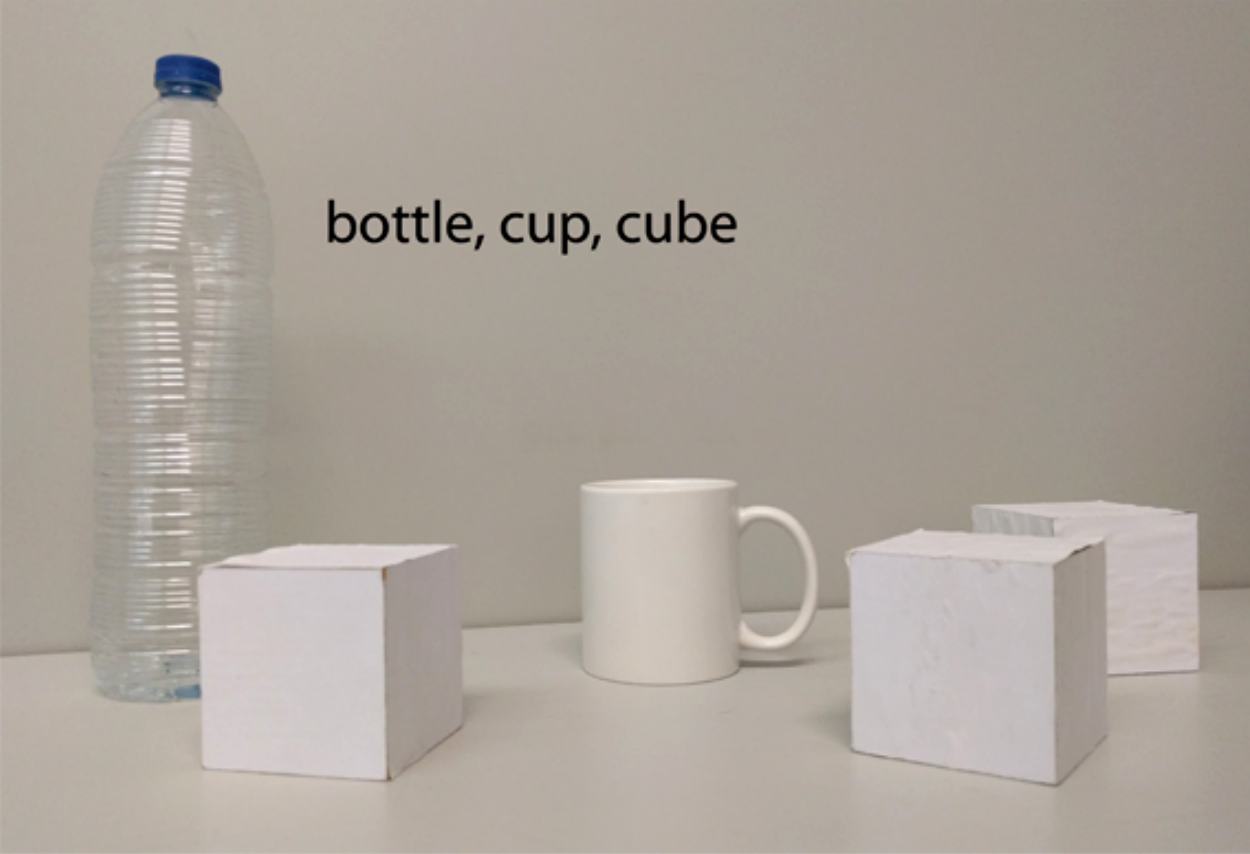
\includegraphics[width=4cm]{images/ch2/fig1_1.png}
    \label{fig1_1}
  }
  \subfigure[Detection (classification + localisation).]{
    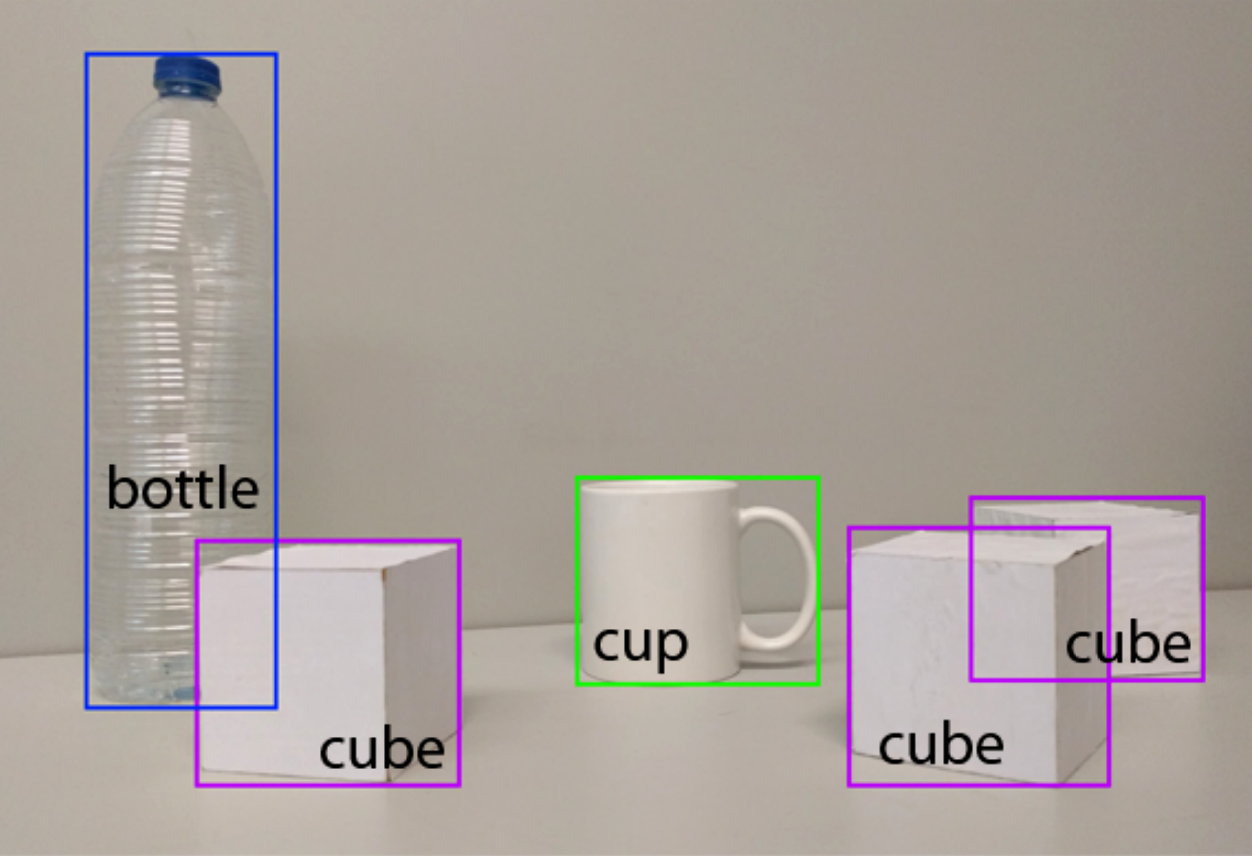
\includegraphics[width=4cm]{images/ch2/fig1_2.png}
    \label{fig1_2}
  }
  
    \subfigure[Image segmentation.]{
    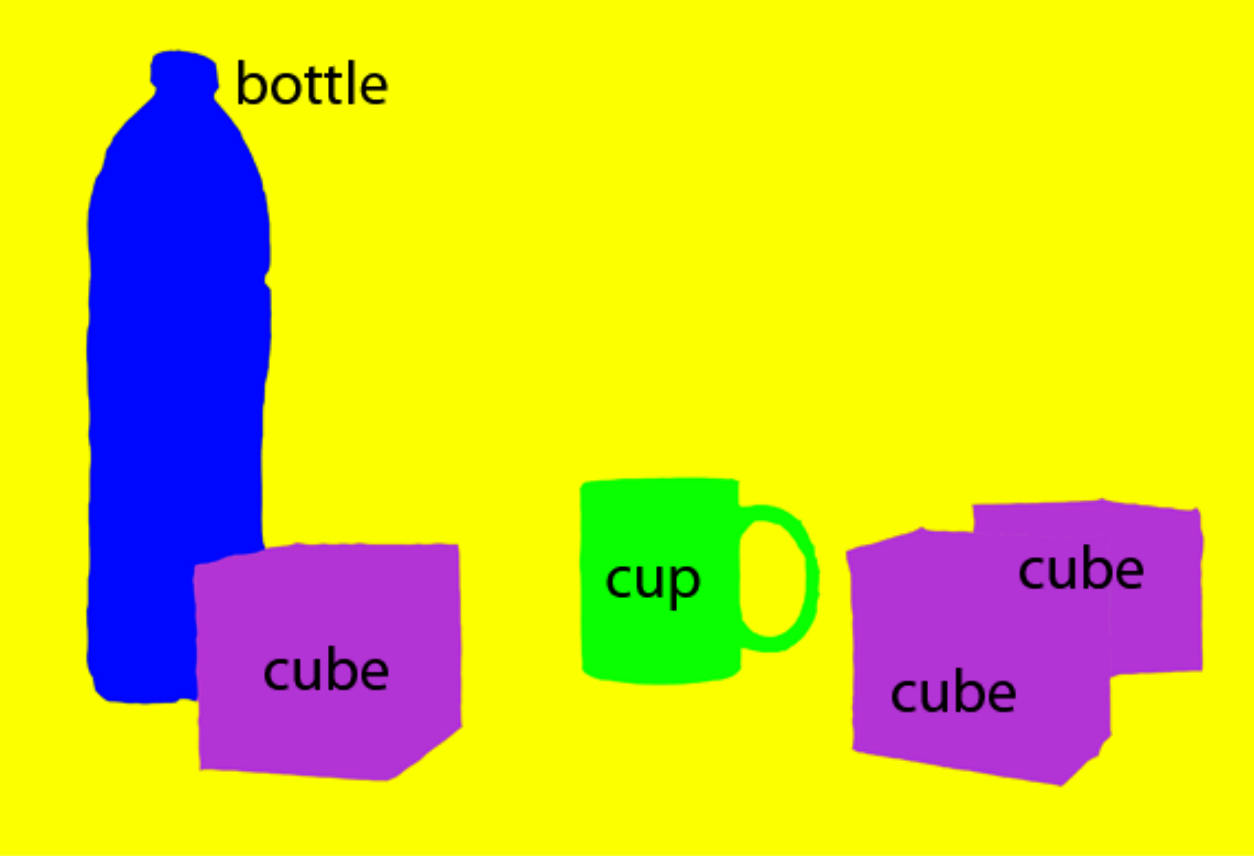
\includegraphics[width=4cm]{images/ch2/fig1_3.png}
    \label{fig1_3}
  }
    \subfigure[Instance segmentation.]{
    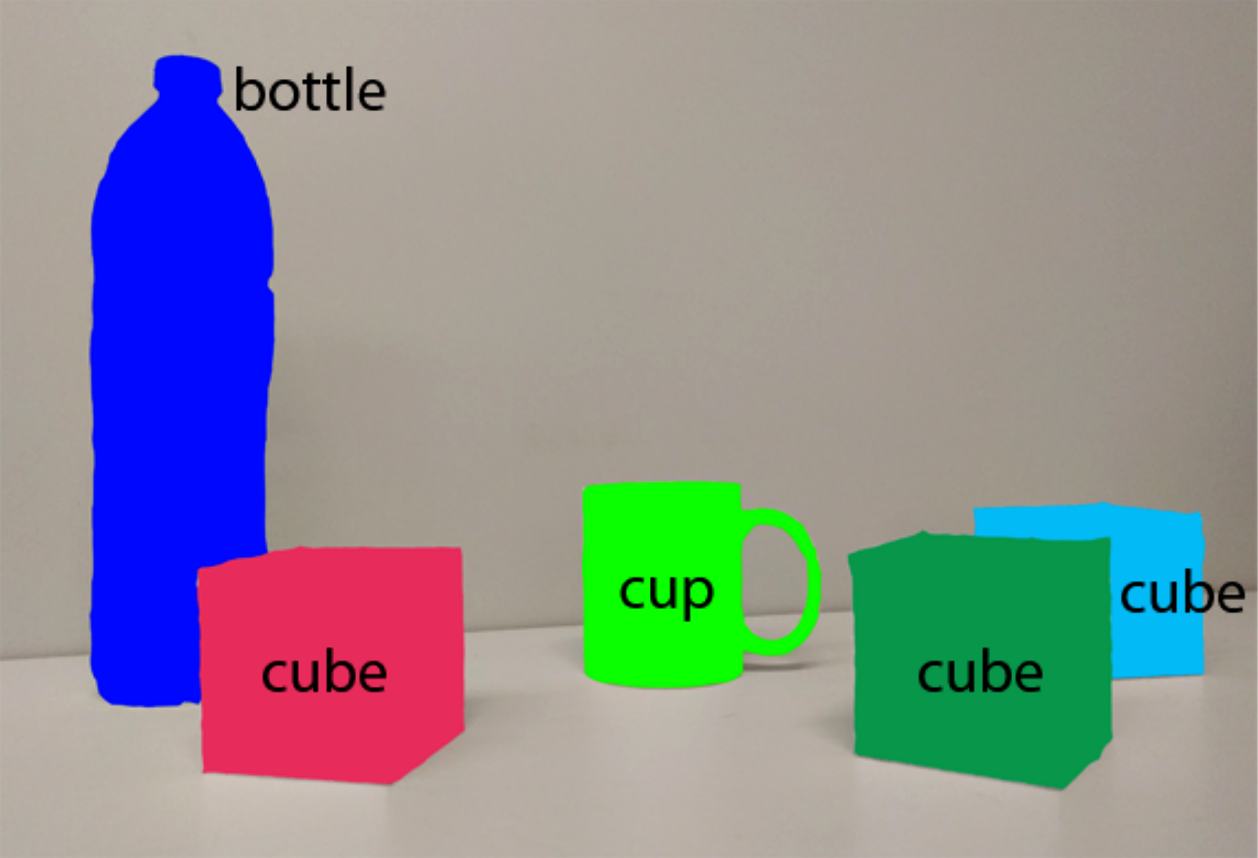
\includegraphics[width=4cm]{images/ch2/fig1_4.png}
    \label{fig1_4}
  }
  \caption{Each task provides semantically richer information (Reproduced from \cite{garcia1704review}).}
  \label{fig1}
\end{figure}

\section{Double-Stage Detectors}

The detection process in double stage or \textbf{\textit{region proposal based detectors}}, can be split in two parts. The first part generates class-agnostic regions of interest (RoIs) with a bounding box around them and the second part predicts the class of each proposed RoI and refines the bounding box around it. It's worth presenting a very popular method in double stage detectors called "R-CNN: Regions with CNN features" (\cite{girshick2014rich}) and its successors Fast R-CNN (\cite{girshick2015fast}) and Faster R-CNN (\cite{ren2015faster}) as Faster R-CNN still stays in fashion due to its high performance.

\subsection{R-CNN}
Before R-CNN was published, object detection was in stagnation without any significant improvement. R-CNN was the first method, that outperformed the previous state-of-the-art CNN method, OverFeat (\cite{sermanet2013overfeat}), increasing accuracy by a big margin. Specifically, R-CNN achieved a mean average precision (mAP) of 31.4\% on ILSVRC2013 (\cite{deng2009imagenet})dataset, over OverFeat which had the previous best result 24.3\%.

R-CNN consists of three parts. The first part generates 2000 class-agnostic regions of interest using selective search (\cite{uijlings2013selective}) with most of them being negative examples. Each proposed region of interest, acts as a potential detection defined by its bounding box. Then, these proposals are warped to a fixed size in order to match architecture's input size criteria. 
The second part is a CNN, pre-trained on the ImageNet dataset (fine-tuned on the new data), and acts as a feature extractor from its last fully connected layer.
The 4096-dimensional extracted features from each RoI, are then classified by class-specific SVMs (plus background) in the last step. After a detection is scored, class-specific box regressors regress the bounding box offsets resulting in a refined bounding box.

\begin{figure}[!htb]
  \centering
  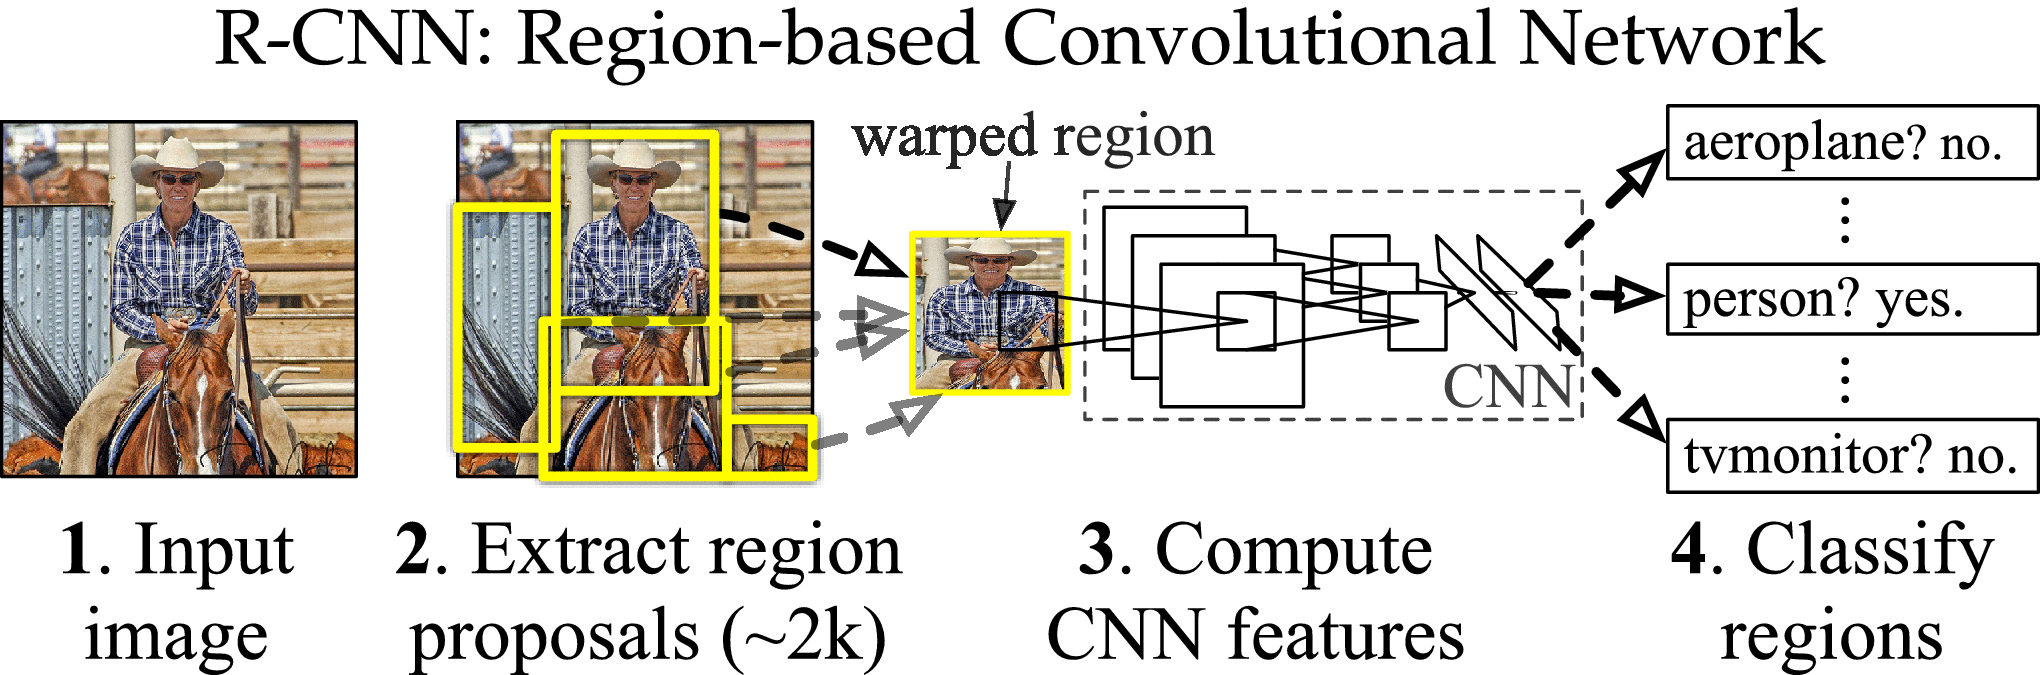
\includegraphics[width=12cm]{images/ch2/fig2.png}
  \caption{R-CNN pipeline as presented in \cite{girshick2014rich}.}
  \label{fig2}
\end{figure}

Although, R-CNN increased performance margin strikingly, has the following notable drawbacks:

\begin{itemize}
  \item The selective search is a heuristic based algorithm, thus it is unable to learn anything during the training procedure. 
  \item Training time takes a vast amount of time and space considering that for each image 2000 proposals have to be fed to the network. Since training it is a multi-stage pipeline, extracted features have to be cached on disk before passed to the SVMs and box regressors. Notice that since the majority of samples are negatives, the authors adopted hard negative mining forcing the model to focus on hard examples (\cite{felzenszwalb2009object}) in order to accelerate convergence.
  \item It is not suitable for real time applications as it has a GPU test rate of  47 seconds/images, when OverFeat was 9x times faster (\cite{girshick2015fast}). 
\end{itemize}

\subsection{Fast R-CNN}
Fast R-CNN was introduced as the improved version of R-CNN, where the multi-stage network was replaced by a single-stage pipeline able to be trained in one stage.

\begin{figure}[!htb]
  \centering
  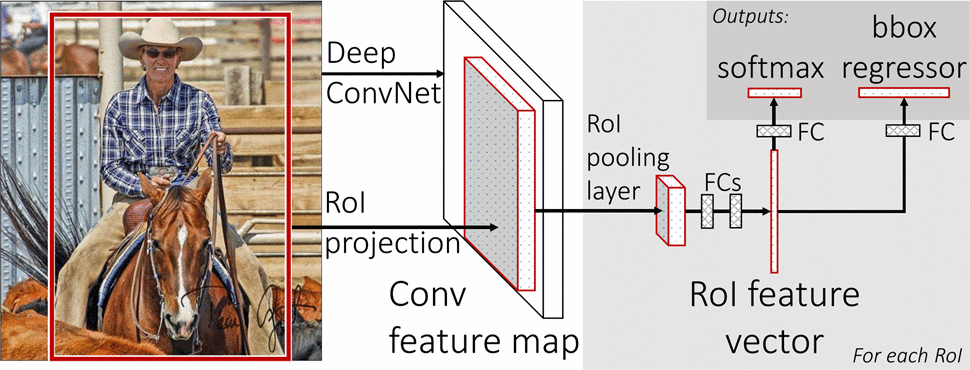
\includegraphics[width=12cm, height=3cm]{images/ch2/fig3.png}
  \caption{Fast R-CNN pipeline as presented in \cite{girshick2015fast}.}
  \label{fig3}
\end{figure}

To achieve this, Faster R-CNN adopted a method from SPPnet (\cite{he2015spatial}) called RoI pooling. R-CNN was handling proposals by warping them into a fixed size and feeding them into the network one by one. On the contrary, SPPnet and Faster R-CNN compute varying size feature maps of the entire image instead of warped region proposals. Each feature map contains RoI information in a four-tuple $(r,c,h,wR-CNN)$, where $r, c:$ top-left corner and $w, h:$ width and height. Fixed size RoI feature vectors are pooled from variable size feature maps through RoI pooling. \fref{fig4} presents how RoI pooling extracts fixed length feature vectors from feature maps with variable sizes. Moreover, the SVMs and the box regressors are replaced by a joint sibling layer. One layer produces the softmax probability over K + 1 background classes, while the other predicts offsets for the refined bounding boxes. \fref{fig3} illustrates an overview of the model. 

\begin{figure}[!htb]
  \centering
  \subfigure[Feature map with 2 RoIs.]{
    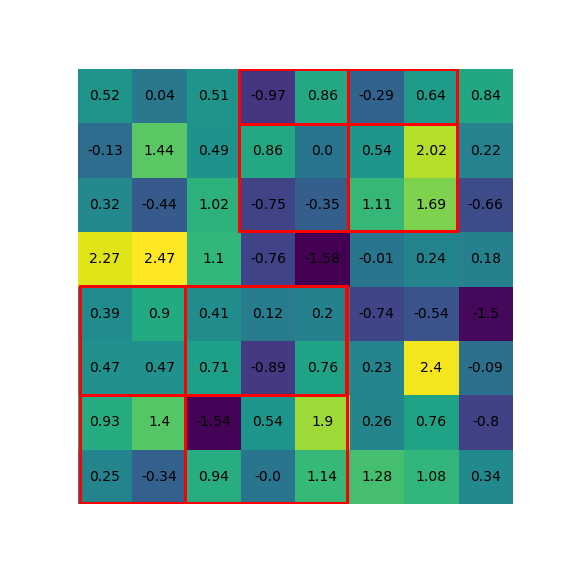
\includegraphics[width=6cm]{images/ch2/fig4_1.png}
    \label{fig1_1}
  }
  \subfigure[RoIs after RoI pooling.]{
    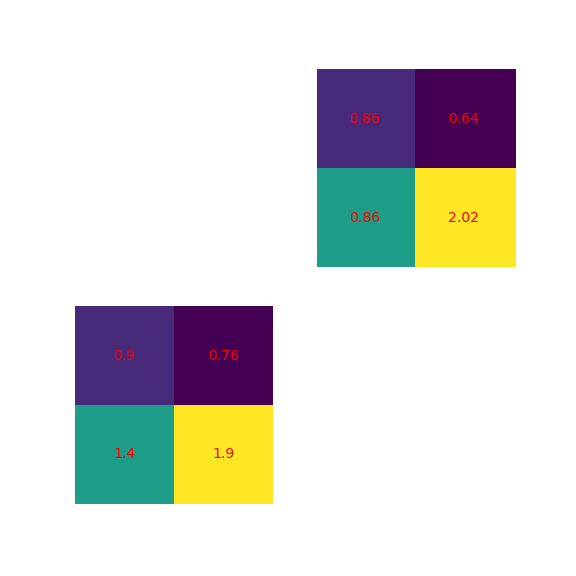
\includegraphics[width=6cm]{images/ch2/fig4_2.png}
    \label{fig1_2}
  }
  \caption{In order to extract vectors of fixed length, different sized proposed RoIs are divided in a fixed number of bins appropriately.}
  \label{fig4}
\end{figure}

By feeding the entire image into the network instead of $\sim$2k proposals one by one, the network avoids redundant computations since a lot of proposals are overlapping each other, hence it is more efficient than its predecessor both in terms of time and memory. Specifically, it is 10x faster than R-CNN in training time and 213x in testing. Furthermore, a joint loss $\mathcal{L}=\mathcal{L}_{cls}+\mathcal{L}_{reg}$ from the softmax and the regression layers optimises the network.

\subsection{Faster R-CNN}
After the replacement of the SVMs with softmax functions, Fast R-CNN was the state-of-the-art object detector, based almost entirely on convolutional neural networks. Its major disadvantage was that the region proposal method, selective search, was not a learning method but a heuristic approach. Soon, this was fixed by the introduction of Faster R-CNN (\cite{ren2015faster}) which entirely dismissed selective search and replaced it with a trainable region proposal network (RPN). RPN, is a CNN where the network's output is attached to a class predictor and a box regressor. The class predictor has only two classes (object, not object), thus the networks is trained to propose regions of interest by their "\textit{objectness}". The rest of the network is adopted by the Fast R-CNN pipeline. Faster R-CNN is classified in the double-stage detectors even if the region proposal method is not decoupled, anymore, from the main pipeline, due to it's 4-step alternate training:
 
\begin{enumerate}
  \item RPN is initialised with the ImageNet weights and fine-tuned for the region proposal task.
  \item The detector (Fast R-CNN) is initialised with the ImageNet weights and fine-tuned for the detection task, with the proposed regions of interest from the RPN (the two models do not share any convolutional layers).
  \item The detector is used to initialise the RPN training, with keeping constant weights coming from shared layers and updating only weights from unique layers. At this point the two models share convolutional layers.
  \item Keeping constant weights from common convolutional layers, detector's unique layers are fine-tuned. 
\end{enumerate}

Faster R-CNN's greatest success is that it consists of a single-stage end-to-end trainable network, entirely based on CNNs with an inference time of 5 FPS.


\section{Single-Stage Detectors}
The downside of double-stage detectors is that training time is split in two separate parts, the region proposal and the detection part, hindering real-time detection. Single-stage detectors or \textbf{\textit{regression/classification based detectors}} have the advantage of being really fast. The main reason is that instead of making class predictions and refining bounding boxes on already proposed regions, apply global rules in every pixel inferring relevant detections without intermediate mechanisms. In this category, the most important algorithms are the SSD (\cite{liu2016ssd}), the YOLO model (\cite{redmon2016you}) and RetinaNet (\cite{lin2017focal}) and will synopsised in the next pages.
 
 \subsection{YOLO}
 YOLO, developed by \cite{redmon2016you} (followed by the improved versions of YOLOv2 \cite{redmon2017yolo9000} and YOLOv3 \cite{redmon2018yolov3}) is a model known for its rapid inference 
 rates ranging between 20-220FPS (depending the backbone implementation) based entirely on Darknet; a network developed by Redmon.
 
 The idea behind YOLO is to obtain detections from each pixel instead of relying on region proposal methods. An image $W\times H$ is fed into the backbone network and the output is an activation feature map of size $S\times S$. Each pixel in the given feature map, represents an area in the original image of $\frac{W}{S} \times \frac{H}{S}$. Also, each cell on the grid is responsible for detecting an object that has its center on that cell. For example, if an object lies in the bottom right corner of the original image, pixel $(S,0)$ on the feature map, is responsible for its detection. If an object lies in the middle of the image, pixel $(\frac{S}{2},\frac{S}{2})$ is responsible for its detection. 
 
\begin{figure}[!htb]
  \centering
  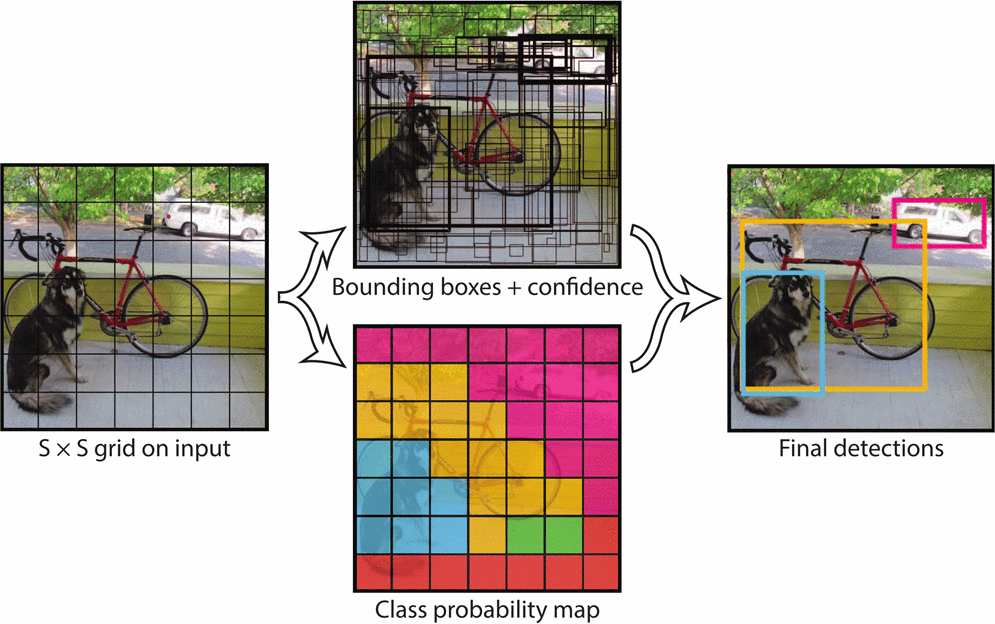
\includegraphics[width=12cm]{images/ch2/fig5.png}
  \caption{A schematic representation of how grid cells detect objects. Reproduced from \cite{redmon2016you}.}
  \label{fig5}
\end{figure} 
 
The actual size of the feature map sized $S\times S$ is a five-tuple $S\times S \times B\times(5+C)$ tensor, where 5 in parentheses implies four coordinates and an objectness score, C is an one-hot encoded vector which indicates the class and B is the number of different detections. As a matter of fact, each cell makes B predictions of arbitrary size and the final detection is the one with the biggest $p_obj$ confidence score. The last layer produces a conditional probability $p(c_i|obj)$ and the refined bounding box.

The next versions of YOLO, could make predictions in intermediate layers (from feature maps of different size) enabling detection in various scales. 
 
\subsection{SSD}
Single Shot Detector (or SSD) was published right after YOLO, by \cite{liu2016ssd} and aimed to solve YOLO problems. SSD follows an architecture based on VGG16 (as Faster R-CNN) and operates as YOLO. The first version of Redmon's detector had difficulties detecting objects in different scales due to multiple pooling layers, thus SSD was aiming to fix this. 

Regarding its architecture, an additional network is attached right after the fifth convolutional block of the VGG16. Classification and regression happens on several feature maps of different size from finer to coarser resolutions. Moreover, grid cells, instead of predicting the conditional class probability $p(c_i|obj)$, predict $p(c_i)$, thus it is necessary the introduction of one more class that acts as background. While SSD could achieved higher mAP than YOLO with similar detection rates and could detect objects in multiple scales, it was facing difficulties in small object detection but this could be relieved by altering the backbone network.  \fref{fig6} shows an overview of the model.
 
\begin{figure}[!htb]
  \centering
  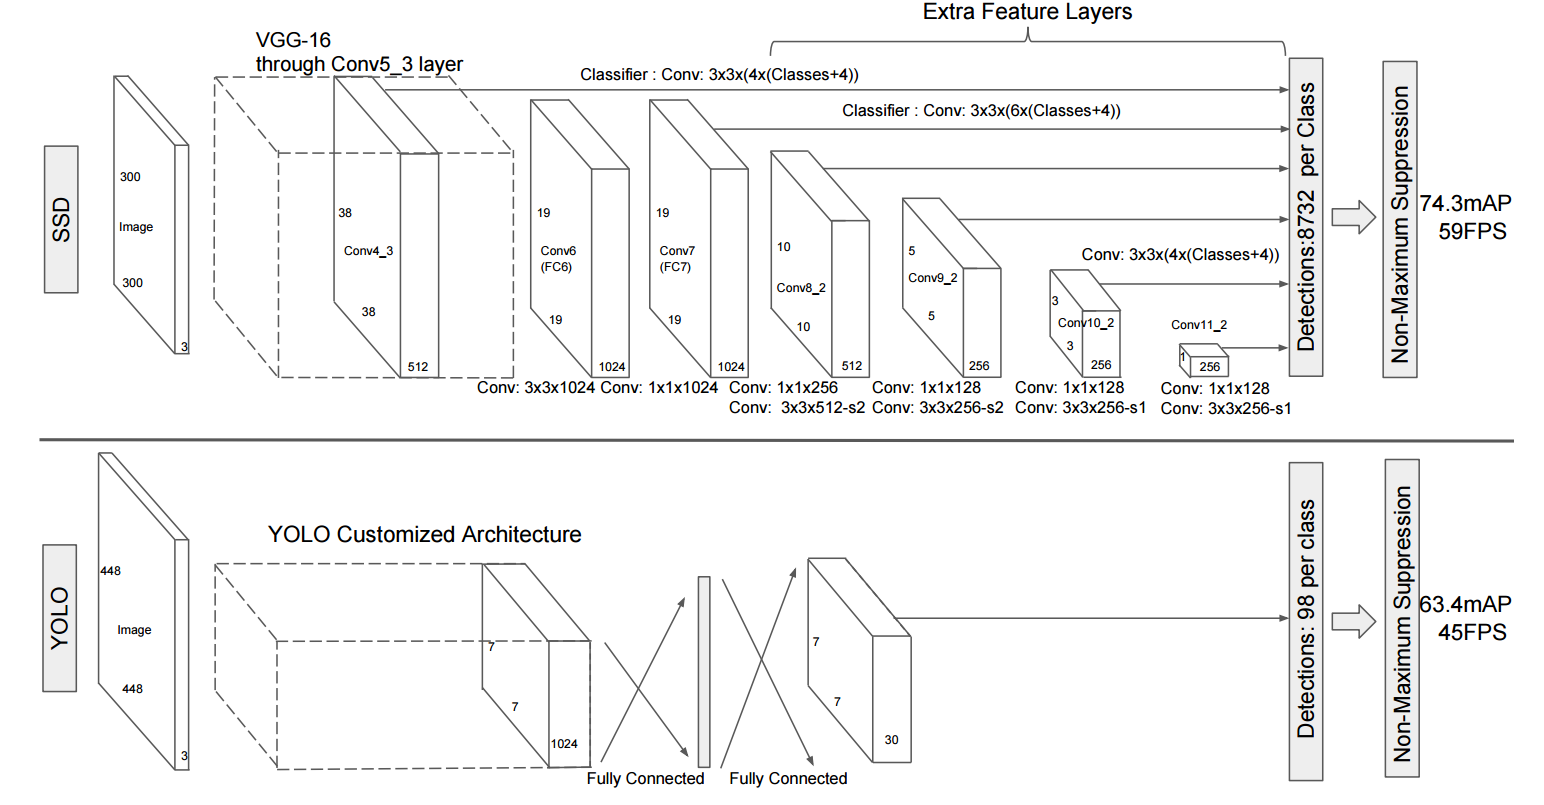
\includegraphics[width=12cm]{images/ch2/fig6.png}
  \caption{A comparison between SSD and YOLO architectures. Reproduced from \cite{liu2016ssd}.}
  \label{fig6}
\end{figure} 
 
The previous sections in this chapter, summarised an overview of the most widely used object detectors, the novelties in their architectures, their advantages along with their shortcomings. One the one hand, double-stage detectors produce region proposals and deal with detection in latter stage, and on the other, single-stage detectors divide the images in a grid and produce a bounding box (or not) around a grid cell depending on a probability $p(obj)$. The trade-off between these object detector families is that double-stage detectors usually achieve higher accuracies, while single-stage detectors are much faster. The following sections provide information about technical specifications and concepts met in every object detector in a more detailed manner.

\section{Prior Bounding Boxes (Anchors)}
Anchors act as reference boxes of predefined size around RoIs; the box regressors on the final layer, try to refine them for an accurate localisation. Instead of producing new coordinates for every detection, predicting the offsets $(\Delta x, \Delta y, \Delta w, \Delta h)$ of the predefined bounding box is much more efficient. These anchor boxes can be more than one with different scales and ratios; in other words, it is easier refining an elongated vertical box around a person rather than a square box. 

Usually, most models define by default 9 anchor boxes with scales of $(2^0, 2^{1/3}, 2^{2/3})$ and ratios of $(1\!:\!2,1\!:\!1,2\!:\!1)$, but this depends on the variation of objects in the dataset. A common practice to find the most representatives scales and ratios is to apply K-means clustering over the dataset.

In single-stage detection, the spatial size of the feature map where the classifier and box predictor are attached to, depends on the depth of the particular convolutional layer. \fref{fig7} shows an $8\times8$ feature map where each grid cell tries to fit best 9 anchor boxes of area $K\times K$. Each grid cell represents a spatial area of $(\frac{W}{8}, \frac{H}{8})$ in the original image. Grid cell $(3,3)$ will make a positive detection if $p(obj)$ is bigger than a certain threshold; if $p(obj)$ on $(4,3)$ exceeds that threshold as well, new prediction's center has 8 pixel distance from the previous. Therefore, this feature map's predictions are characterised by a stride = 8. More dense predictions can be achieved by feature maps of bigger spatial size. Hence pooling layers have a direct effect on prediction density.

 \begin{figure}[!htb]
  \centering
  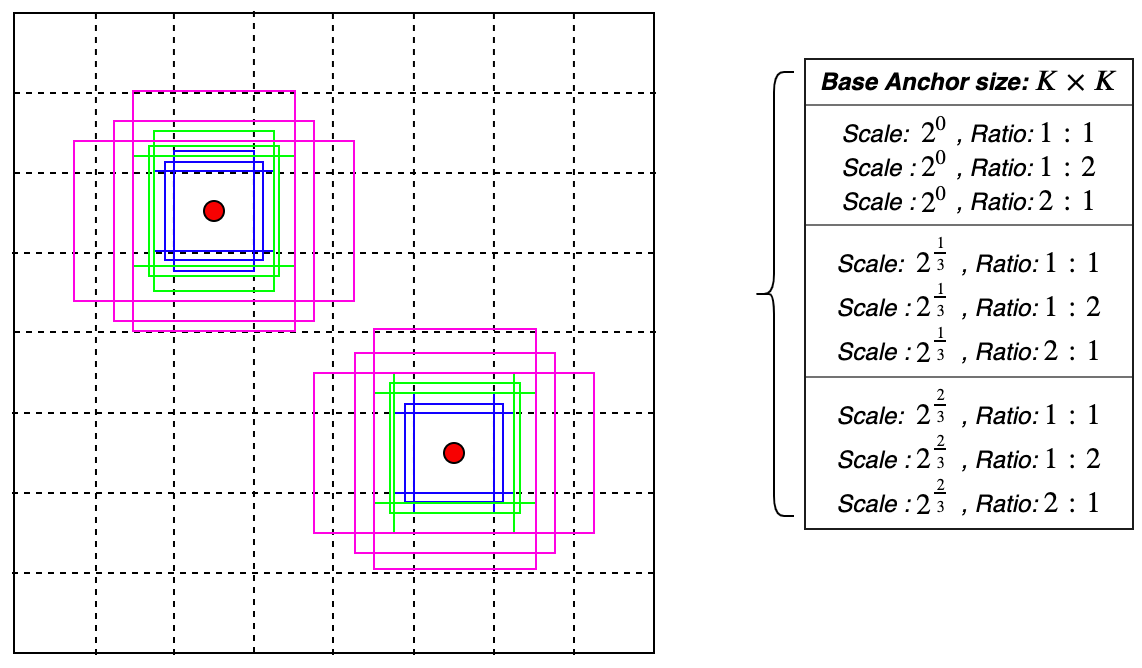
\includegraphics[width=7cm]{images/ch2/fig7.png}
  \caption{A typical topology with 9 anchors acting as prior bounding boxes.}
  \label{fig7}
\end{figure} 

In order to associate ground truth boxes with suitable anchors, each anchor gets assigned with the overlap between the anchor and the ground truth box that covers the most (if any). If the IoU overlap is more than 0.5, then this anchor should detect the object and it's called \textbf{\textit{positive anchor}}. If the IoU overlap is less than 0.4, that anchor should not make a a prediction and it's classified as a \textbf{\textit{negative anchor}}. During training, if an anchor is neither positive nor negative, it does not contribute to the overall loss. In inference mode, only the anchor with the biggest overlap will be proposed.

\section{Intersection Over Union}
Intersection over Union or Jaccard index, is an evaluation metric used to measure how accurately a predicted box match or overlaps the ground truth. As name indicates, the ratio between the intersection and the union of two boxes. In most tasks, as in PASCAL VOC challenge \cite{everingham2010pascal}, if the IoU between the detection and the ground truth is more than 0.5, the detection counts as a true positive.

\begin{figure}[!htb]
  \centering
  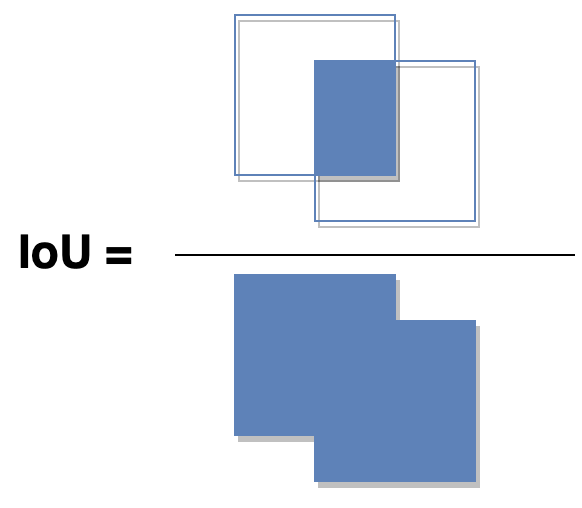
\includegraphics[width=3cm]{images/ch2/fig8.png}
  \caption{The Intersection over Union ratio.}
  \label{fig8}
\end{figure} 

\section{Non-Maximum Suppression}
Usually, objects extend much more in space rather than occupying only a grid cell on the feature map. Thus, many adjacent grid cells, by processing similar context information, may be triggered and produce multiple predictions referring to the same object. A post processing technique called non-maximum suppression (NMS) deals with this problem by suppressing the detections with IoU over a certain threshold. NMS algorithm can be summarised in the following steps:

\begin{itemize}
  \item In each cell, if $p(obj)>obj_{th}$ the anchor with the biggest IoU with the ground truth box will be proposed as prediction. 
  \item If there are overlapping predictions, with IoU greater than $NMS_{th}$, the detection with the highest $p(c_i|obj)$ will be proposed as the prediction, while the remaining predictions with be suppressed. 
\end{itemize}

That way NMS suppresses multiple predictions that most likely refer to the same object, but if there are objects that are really close to each other, and their detections have possibly an overlap greater than $NMS_{th}$, most of them will be falsely suppressed but one. 

\section{Multi-task Loss} 
\cite{ren2015faster}, in Faster R-CNN, introduced a coupled loss which combined both the loss from the classification and the regression task. During training, only positive and negative anchors contribute to the loss function; positive anchors in both classification and regression task while negatives only in classification.
The multi-task loss is a weighted combination of the smooth L1 loss and cross entropy.

\begin{equation}
  L(p_i,t_i) = \frac{1}{N_{cls}}\sum_i{L_{cls}(p_i,p_i^*)}+ \frac{\lambda}{N_{reg}}\sum_i p_i^*{L_{reg}(t_i,t_i^*)}
\end{equation} 

$N_{cls}$, and $N_{reg}$ are normalisation parameters, usually the number of instances in the SGD sample and $\lambda$ a balancing parameter. $p_i^*, p_i$ indicates the ground truth and predicted probability respectively, while $t_i^*, t_i$ is a four-tuple referring to the 4 ground truth and predicted coordinates that describe the bounding box.

\begin{equation}
    L_{cls}(p,p^*)= \bigg\{
    \begin{array}{ll}
      -log(p) & \text{if } p^*=1 \\
      -log(1-p) &  \text{otherwise}\\
    \end{array}
\end{equation}

Smooth L1 loss is claimed to be more robust to outliers (\cite{ren2015faster}) rather than L2 in which inappropriate learning rates result in exploding gradients. For similar values, or when the manhattan distance between $t_i, t_i^*$ is very small, smooth L1 is much smaller than L1. Additionally, for L1 greater than 1, it can be seen that gradients are constrained to 1. SSD uses the default formula for smooth L1 loss while Faster R-CNN adopts a parameter $\sigma$ which control the point between quadratic and linear loss. Large values of $\sigma$ convert smooth L1 loss to L2 loss.

\begin{equation}
    L_{reg}(t,t^*)= \bigg\{
    \begin{array}{ll}
      0.5\sigma^2(t-t^*)^2 & \text{if } |t-t^*|\leq \frac{1}{\sigma^2} \\
      |t-t^*|-\frac{0.5}{\sigma^2} &  \text{otherwise} \\
    \end{array}
\end{equation}

The following equations show the adopted parameterisation for $t_i$, where $(x^*,y^*,w^*,h^*)$, $(x_a,y_a,w_a,w_h)$ and $(x,y,w,h)$ refer to ground truth, anchor and predicted boxes respectively. 

\begin{align}
t_x		&= (x-x_a)/w_a			&		t_y	&= (y-y_a)/h_a \\
t_w		&= log(w/w_a)			&		t_h 	&= log(h/h_a) \\
t_x^*		&= (x^*-x_a)/w_a		&		t_y^*	&= (y^*-y_a)/h_a \\
t_w^*	&= log(w^*/w_a)		&		t_h^*	&= log(h^*/h_a) 
\end{align}

\section{Focal Loss}
The number of bounding box priors covering the image, is usually very large, orders of magnitude greater than the number of instances in the image. This creates a class imbalance between negative and positive anchors. To address this class imbalance, \cite{lin2017focal}, introduced a weighted cross entropy loss named "focal loss". Prior to focal loss, the most widely adopted method to deal with class imbalance was Online Hard Example Mining explicitly showing the model the hard examples to calculate gradients according to them. Another strategy is feeding the model with a sampling ratio of 1:3 in positives and negatives samples.

Focal loss, down-weights cross entropy asymmetrically forcing the model to focus on hard examples, that is examples with low confidence $p$. $\gamma$ is the scaling factor, and $\alpha_t$ a balancing factor, the authors state that its precise form is not crucial.

\begin{equation}
    FL(p,p^*)= \bigg\{
    \begin{array}{ll}
      -a_t(1-p)^\gamma log(p) & \text{if } p^*=1 \\
      -a_tp^\gamma log(1-p) &  \text{otherwise}\\
    \end{array}
\end{equation}

\section{RetinaNet}
RetinaNet, was introduced as a single-stage adaptation of the Feature Pyramids Networks (FPN, \cite{lin2017feature}) with the enhancement of focal loss. It is the bridge between double-stage and single-stage detection, as it surpassed the performance of Faster R-CNN with detection rates similar to YOLO and SSD.

Detecting objects in different scales is a demanding task and the standard approach is using image pyramids as a solution. SSD made one of the first attempts in multi-scale object detection by exploiting network's pyramidal feature hierarchy. A convolutional network has the advantage of producing, in each layer, feature maps that get semantically richer with the depth of the layer. Pooling operations, result in feature maps, large in resolution but weak in information and more coarse feature maps but semantically rich, obtained from the deeper layers. RetinaNet exploits feature maps from intermediate network layers by combining large resolution semantically weak features with coarser, semantically stronger feature maps. \fref{fig9}, shows different types of pyramidal feature exploitation.

\begin{figure}[!htb]
  \centering
  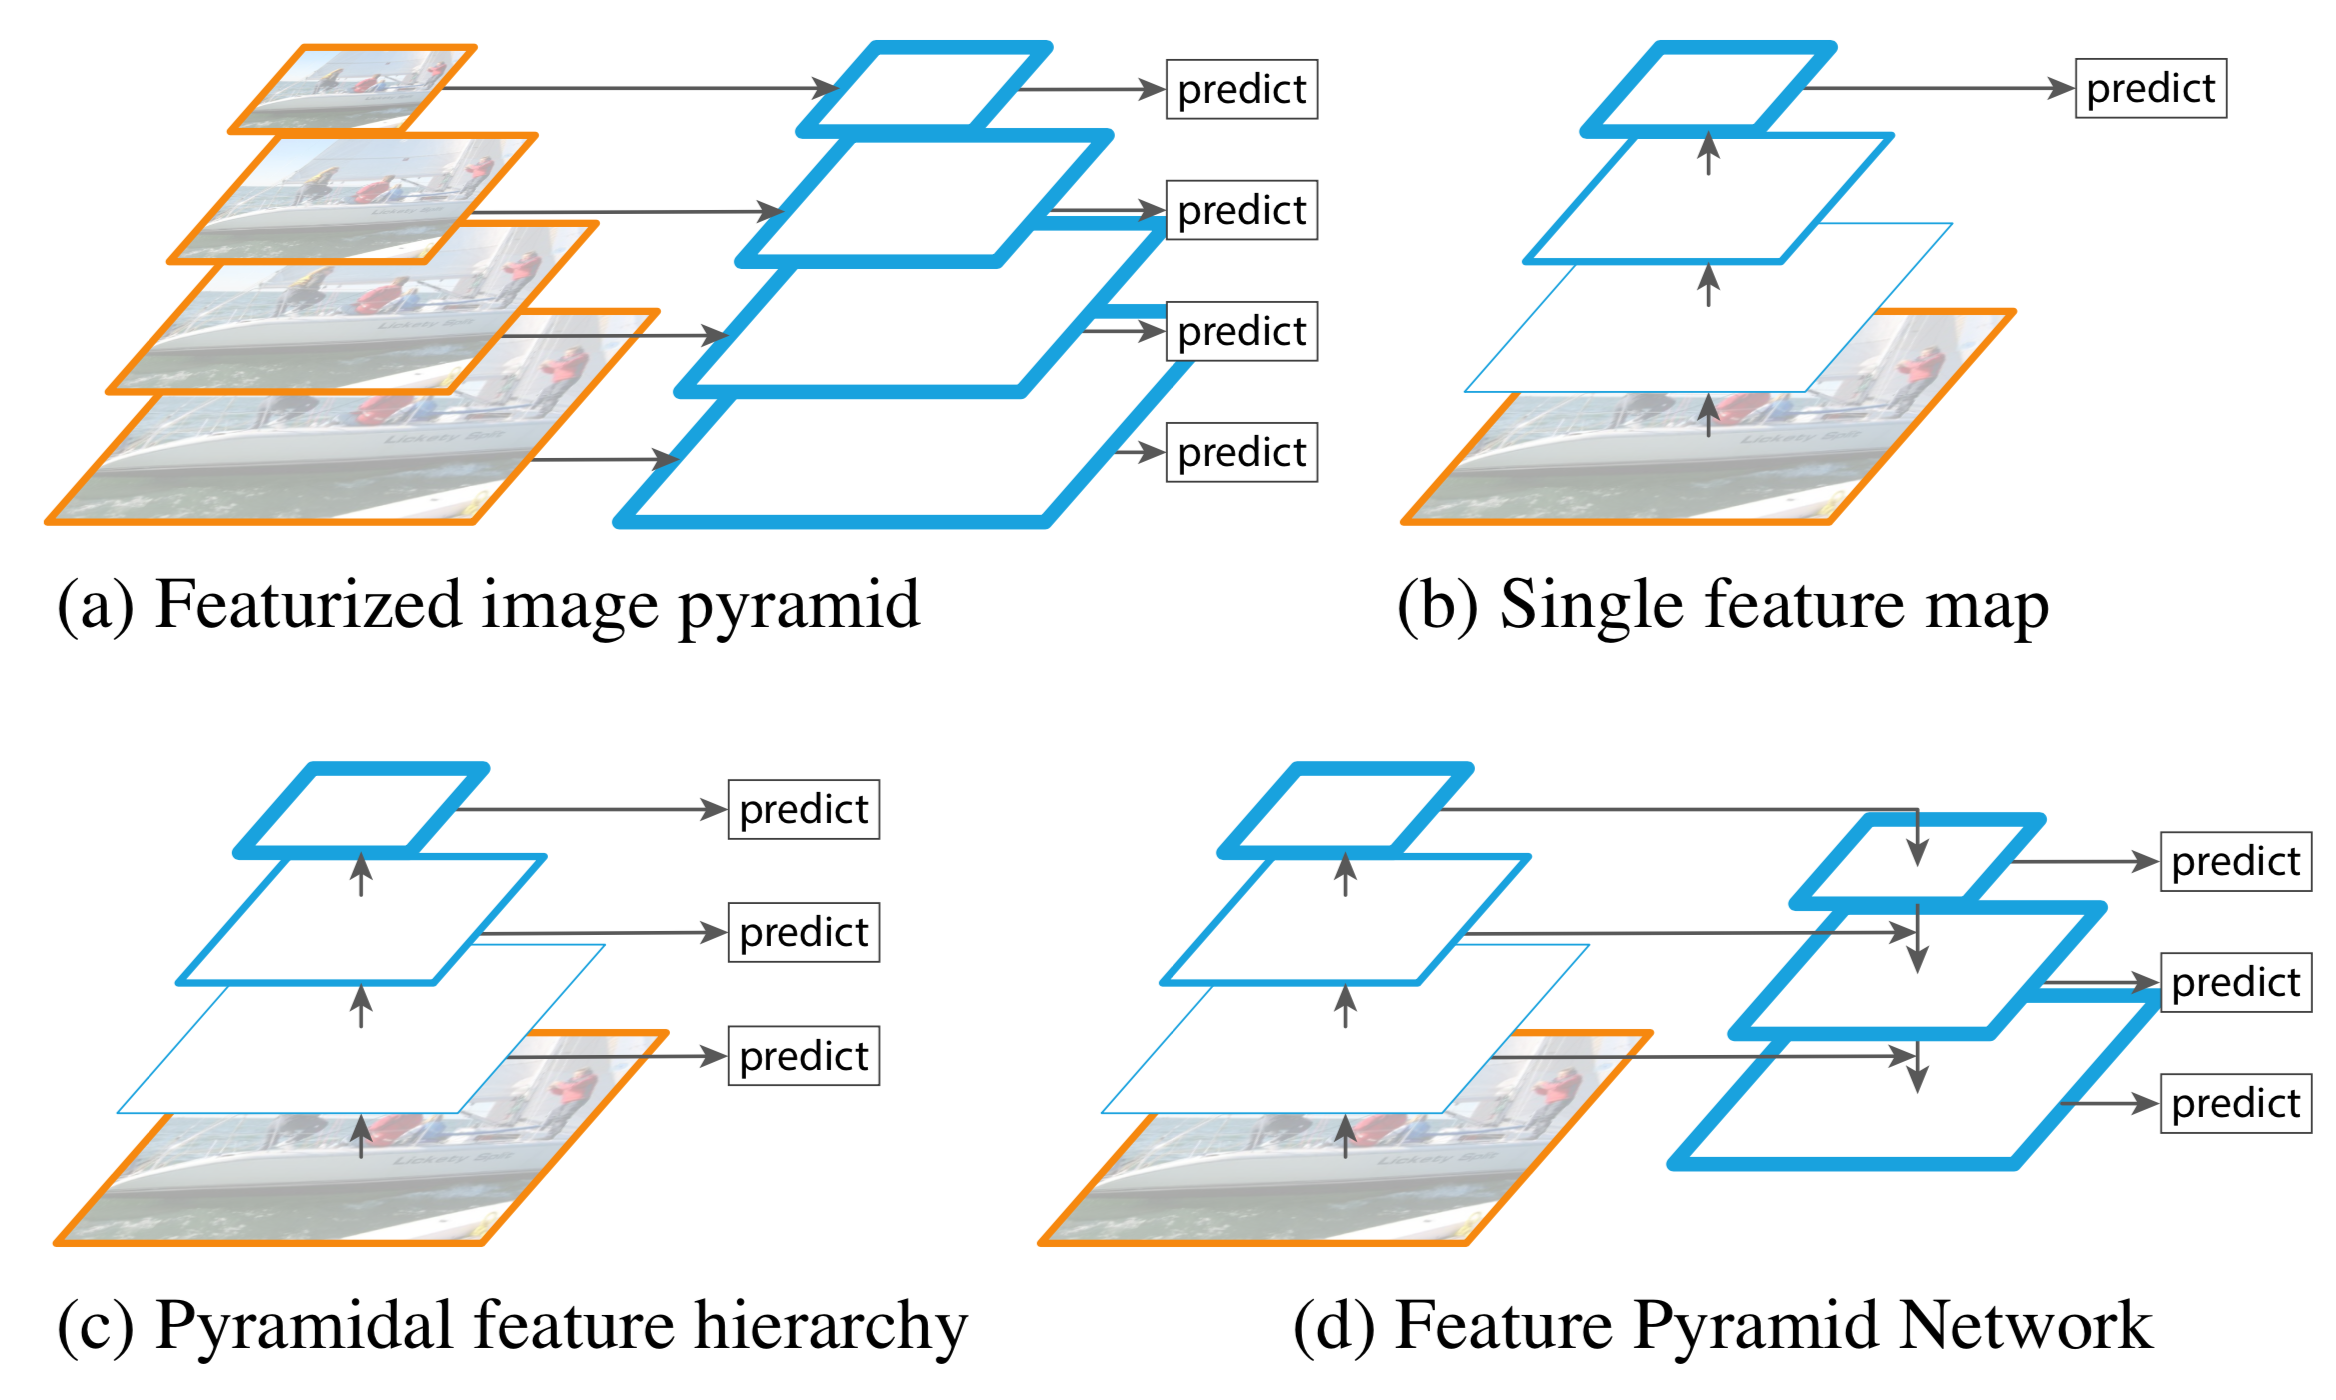
\includegraphics[width=12cm]{images/ch2/fig9.png}
  \caption{(a) Building an image pyramid by feeding an image in multiple scales, this is used to be a common practice but it is computationally infeasible. (b) Feeding an image and making predictions from the coarsest, very rich in information, feature map. It is a very fast method for making single scale predictions. (c) Detection in different scales by exploiting feature maps in the intermediate layers; it was adopted by the SSD. (d) The FPN method. Detects objects in different scales as a common SSD detector, but bottom layers are enriched with upsampled coarser, semantically stronger, top layers. Reproduced from \cite{lin2017feature}}
  \label{fig9}
\end{figure} 

\subsection{Architecture}
\fref{fig10} shows how the spatially larger feature maps are enriched by adding upsampled coarser maps. During the bottom-up pathway, the backbone network computes feature maps at several scales with the help of pooling operations. In the case of the VGG architecture, the model consists of 5 convolutional blocks and in the end of each convolutional block, the feature map is downscaled by 2 (the depth of the feature map depends on the architecture) resulting in the hierarchical features $(C_1, C_2, C_3, C_4, C_5)$. For the top-bottom pathway, the feature maps $C_i$ are obtained via lateral connections and convolved with $1\times1$ kernels to produce $C_{i_{reduced}}$ features of the same spatial size but with fixed depth. The coarser feature map is upsampled by the nearest neighbour method, and is added element-wisely with the $C_{i_{reduced}}$ maps. Each merged map, finally undergoes a $3\times3$ convolution to reduce the aliasing effect from upsampling. The result is a set of features downscaled by 2, $(P_1,P_2,P_3,P_4,P_5)$, where each $P_i$ contains information from deeper level features. 

\begin{figure}[!htb]
  \centering
  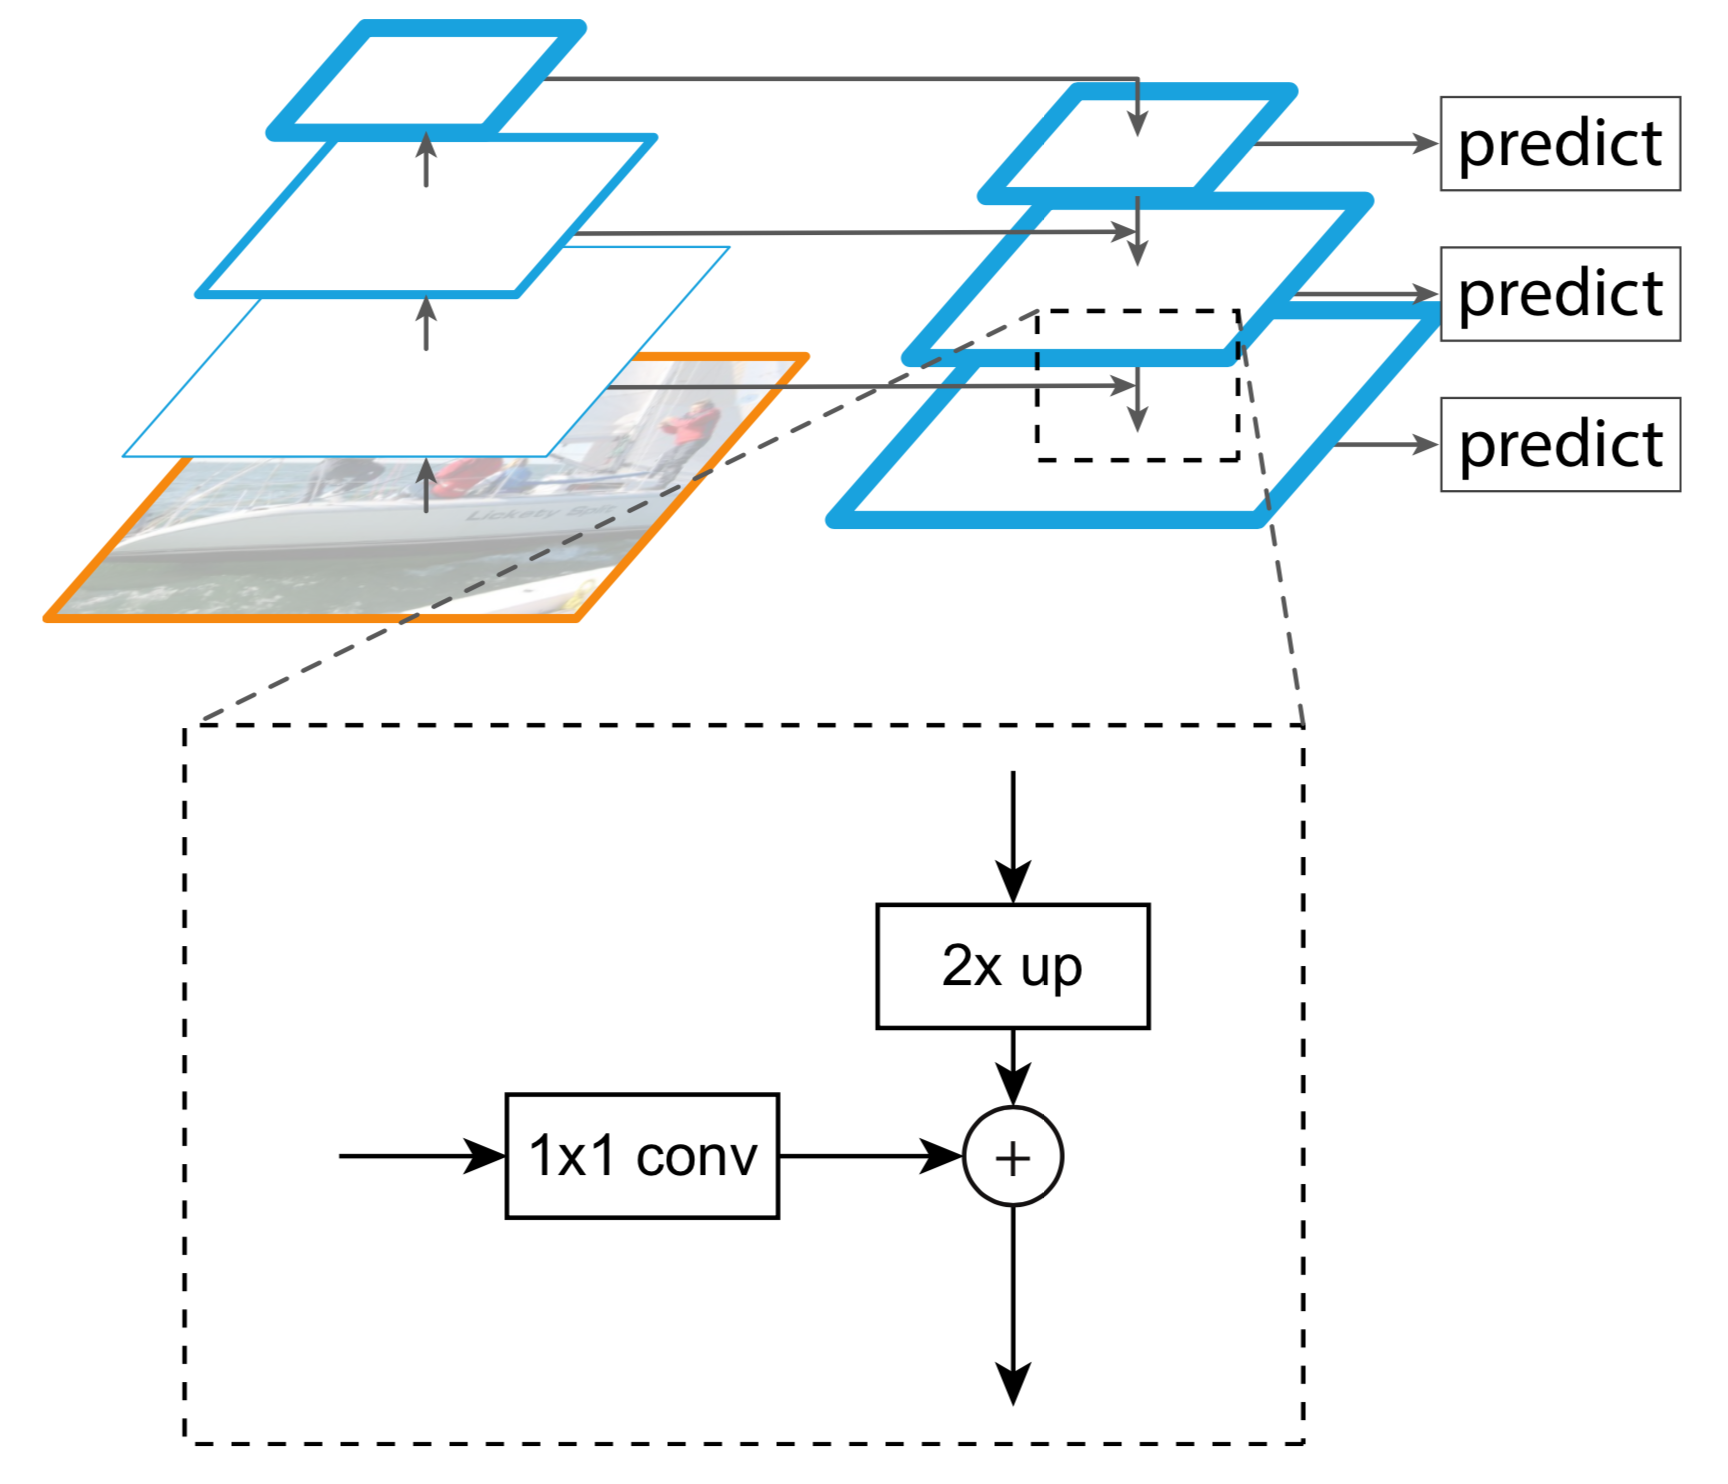
\includegraphics[width=6cm]{images/ch2/fig10.png}
  \caption{Top-down building block in RetinaNet and FPN. Reproduced from \cite{lin2017feature}}
  \label{fig10}
\end{figure} 

In fact, instead of featurising the output layers in each convolutional block, RetinaNet, attaches in the end of the backbone network two more \textbf{$3\times3$ strided convolutional layers}, continuing downscaling by the same factor the output, without making use of pooling. These outputs are noted as $C_6,C_7$ and the featurised levels are the set $(C_3, C_4, C_5, C_6, C_7)$ which produce the output pyramidal layers $(P_3, P_4, P_5, P_6, P_7)$.

\subsection{Anchor boxes}
RetinaNet, adapts the anchor boxes concept to produce RoIs in contrast with the FPN which uses a region proposal network. Due to the number of pooling operations every pyramidal level has underwent, the stride in each $P_i$ layer is $(8, 16, 32, 64, 128)$\footnote{$P_3$ has already been pooled 3 times from block$_1$, block$_2$ and block$_3$, thus it has a stride of $2^3$.}. The effective receptive field of each layer is crucial and act as a limiting factor for the size of the anchors and the size of the detected object as a consequence; stride on the other hand, indicates the density of the predictions. However, in RetinaNet this is not completely true as each $P_i$ is product of many layer outputs, from various depths with different receptive fields. In general, spatially large $P_i$ features aim in dense small object detection, while coarser $P_i$ maps are responsible for large object detection. Specifically, each layer has anchors in three scales and three ratios. Anchor's base size is $(32^2, 64^2, 128^2, 256^2, 512^2)$ with scales $(2^0, 2^{1/3}, 2^{2/3})$ and ratios of $(1\!:\!2,1\!:\!1,2\!:\!1)$.

\subsection{Prediction subnet}
The subnetwork responsible for detections consist of a \textbf{classification subnet} and a \textbf{box regression subnet}. The classification subnet predicts $p(c_i)$, out of K classes, in each anchor position and is nothing more than 4 stacked $3\times3\times C$ convolutional kernels with ReLU activations, followed by  $3\times3\times KA$ with sigmoid activation. C is the channel depth of $P_i$ and is the same all layers.

The class agnostic box regression subnet, follows the same logic with 4 stacked $3\times3\times C$ convolutional kernels with ReLU activations, followed by $3\times3\times 4A$ with sigmoid activation. The output is a four-tuple for every anchor position with the refined bounding box. The prediction subnet shares its parameters across all pyramidal $P_i$ outputs, following the same philosophy as SSD.

\section{Evaluation Metrics}
Object detection has several evaluation metrics, however performance comparisons depend on the problem. For example in the PASCAL VOC challenge, models compete between those with the highest mAP, while in the apple detection problem a model with higher F1-score is more accurate. However the most useful metrics are:

\bigskip
\textbf{Recall}
\bigskip\noindent
\begin{equation}
  \text{Recall} = \frac{TP}{TP+FN}=\frac{TP}{\text{Num. of objects}}
\end{equation} 
Recall is the fraction between successfully detected instances and the number of instances.

\bigskip
\textbf{Precision}
\bigskip\noindent
\begin{equation}
  \text{Precision} = \frac{TP}{TP+FP}=\frac{TP}{\text{Predictions}}
\end{equation} 
Precision gives the ability of the model identifying only the relevant instances as it gets lower for every wrong prediction.

\bigskip
\textbf{F1-score}
\bigskip\noindent
\begin{equation}
  \text{F1-score} = 2\times\frac{\text{Precision}\times \text{Recall}}{\text{Precision}+\text{Recall}}\end{equation} 
F1-score is the harmonic mean between precision in recall, giving equal importance in both. It is mostly used in tasks where the model should find the best ratio between true positives and false positives. Changing detector's confidence threshold comes with an expense in the rate of true positives along with the rate of false negatives. F1-score indicates the point in the precision-recall curve where precision and recall have the maximum values.

%\bigskip
%\textbf{Average Precision}
%\bigskip\noindent
%Average precision is the area under curve (AUC) of the precision - recall curve. The PR curve follows usually a zigzag pattern complicating its calculation. \cite{everingham2010pascal}, proposed an alternative way in its calculation by interpolating precision in 11 evenly space points. The precision at each recall level takes the maximum value in order to eliminate the zigzag pattern.
%\begin{equation}
%  \text{AP} = \frac{1}{11}\sum_{r\in\{0,0.1,...,1\}}p_{interp}(r) \\
%  p_{interp}(r)=\max_{\hat{r}:\hat{r}\geq r}p(\hat{r})
%\end{equation} 
\dots
%% ----------------------------------------------------------------
%% Experiment.tex
%% ---------------------------------------------------------------- 
\chapter{RetinaNet Deployment And Proposed Architectures} \label{Chapter:Experiment}
This chapter presents a detailed and analytical description of the system deployment, the proposed architectures and the hyper-parameter selection accompanied by the respective reasoning behind every choice. It is also investigated, how performance scales in function with the dataset training size. Finally, peak detection and counting is achieved by optimising the hyper-parameters of the final pipeline.

\section{Dataset Description}
The dataset used in the present thesis, was released in the work of \cite{bargoti2017image} and \cite{bargoti2017deep} and is provided through the Australian Centre or Field Robotics (ACFR), The University of Sydney\footnote{\url{http://data.acfr.usyd.edu.au/ag/treecrops/2016-multifruit/}}. The images were collected using the platform "Shrimp", an unmanned ground vehicle in apple, mango and almond orchards. However, in this study, only the apple subset is used.

Specifically, the dataset consists of random crops from images that span entire trees, trellised in the orchard block. The total number of apple instances in the images represents the total number of fruits in the orchard block. The split in training, validation and test set follows the proposed split from authors' previous work, to provide valid comparisons with the previous literature work. An overview of the dataset is presented in \tref{tab1}.

\begin{table}[!htb]
  \centering
  \resizebox{\textwidth}{!}{
  \begin{tabular}{cccccc}
  \toprule
  \textbf{Set} & \textbf{Raw Img. Size} & \textbf{Cropped Img. Size} & \textbf{No. of Img.} & \textbf{Fruit Width} & \textbf{Fruits/Img.} \\
  \midrule
  train 		& $1616\times1232$ & $202\times308$ & 896	& $36.27 \pm 7.55$  & $5.22 \pm 3.37$\\
  val. 		& $1616\times1232$ & $202\times308$ & 112 	& $35.92 \pm 7.83$  & $4.80 \pm 3.10$\\
  test. 		& $1616\times1232$ & $202\times308$ & 112 	& $35.29 \pm 7.30$  & $4.95 \pm 3.21$\\
  train + val. 	& $1616\times1232$ & $202\times308$ & 1008	& $36.23 \pm 7.58$	& $5.17 \pm 3.35$\\
  \bottomrule
  \end{tabular}
  }
  \caption{ACFR dataset description}
  \label{tab1}
\end{table}

The dataset provides circular annotations for the fruits; thus, they were converted to squares with the same width and height. Instead of discarding annotations that exceed the borders of the image, they were clipped to fit the image.
 
 \begin{figure}[!htb]
  \centering
  \subfigure[]{
    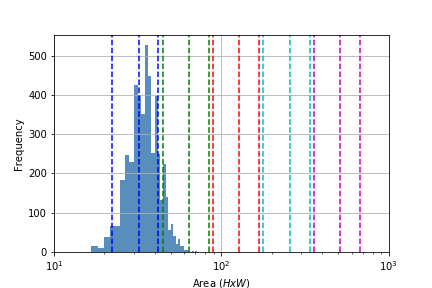
\includegraphics[width=0.30\textwidth]{figures/ch3/fig1_1.png}
    \label{fig1_1}
  }
  \subfigure[]{
    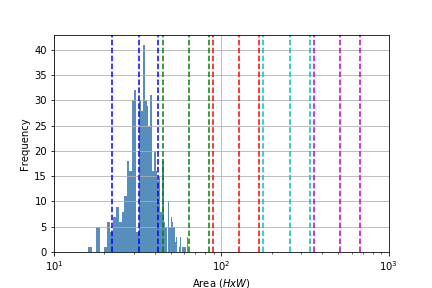
\includegraphics[width=0.30\textwidth]{figures/ch3/fig1_2.png}
    \label{fig1_2}
  }
  
    \subfigure[]{
    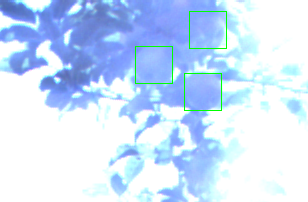
\includegraphics[width=0.30\textwidth]{figures/ch3/fig1_3.png}
    \label{fig1_3}
  }
  \subfigure[]{
    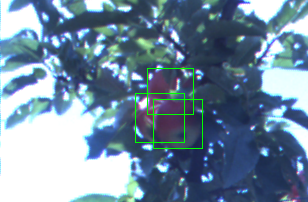
\includegraphics[width=0.30\textwidth]{figures/ch3/fig1_4.png}
    \label{fig1_4}
  }
  \caption{Typical samples from the ACFR dataset: A sample with (a) well-separated apples, (b) some unannotated instances and 
  		(c) poor lighting conditions. (d) NMS suppresses all predictions with $\text{IoU}\geq\text{NMS}_{th}$ apart from the one with the biggest confidence.}
  \label{fig1}
\end{figure}
 
\section{Proposed Deployment and Configuration}
\subsection{Hardware and Software specifications}
The deployment was set up on the Keras (\cite{chollet2015keras}) implementation of RetinaNet, provided by Fizyr\footnote{\url{https://github.com/fizyr/keras-retinanet}} and trained using a single NVIDIA GeForce GTX 1080 Ti provided by the Iridis 5\footnote{\url{https://www.southampton.ac.uk/isolutions/staff/iridis.page}} Computer Cluster. The repository with detailed instructions can be found in \url{https://github.com/nikostsagk/Apple-detection}.

\subsection{Training Details}\label{training_details}
All models were trained on the complete training set, consisting of 896 images, while performance was monitored with respect to the validation set. Performance metrics presented below refer to the test set.

The models were trained for 30 epochs of 2000 steps each with $\text{batch size} = 1$. Regarding the optimiser, ADAM (\cite{kingma2014adam}) was used, with an initial learning rate of $10^{-5}$, decreased later by a factor of 10 on epoch 15 and again on 25. It was observed that the models did not exhibit any signs of overfitting as the performance on the validation set was increasing until it stabilised around its maximum value; meanwhile, the validation loss was fluctuating around a minimum value. All models were initialised on the ImageNet VGG16 pre-trained weights unless otherwise stated. 30 epochs of training time took around 80-90 minutes for each model, but the performance had reached its peak from the first 6 epochs.

\subsection{Data Augmentation \& Preprocessing}
Originally, RetinaNet was trained on images with a minimum side of 800. Therefore, first tries adopted this strategy, keeping the ratio unchanged (e.g. $800\times1220)$. Later, a resolution of $512\times781$ was proposed, in order to save training and inference time, ensuring at the same time that at least one pixel can represent a fruit in the last layer (P7). Finally, the resolution utilised in all models was the original $202\times308$ as no model showed any gain in performance with higher resolutions. By adopting the original resolution, there are considerable benefits in training and inference time, allowing training multiple models.

The data augmentation techniques used were along with the natural variations of the dataset. Specifically, the augmentations included random flipping along the x-axis with 0.5 chance and random photometric transformations such as \textit{Fancy PCA} (as described in \cite{taylor2017improving}), changes in brightness/contrast and changes in the HSV colour space. Instead of expanding the dataset before training begins, each sample is randomly transformed during training, avoiding pre-calculations. Besides the augmentation, the ImageNet mean values were subtracted from the dataset, as the VGG16 was initially trained that way.

\subsection{Anchor Boxes Configuration}
Instead of using the default anchor boxes' base size, ratios and scales, a common practice used in anchor-based detection pipelines (\cite{redmon2017yolo9000}, \cite{redmon2018yolov3}) is k-means clustering. The dataset is divided in $k$ clusters, where the $k$ centroids' width and height define anchors' base size. Nonetheless, this practice cannot be adopted in the present dataset. In such case, all anchors would have similar dimensions, due to the very small variance among the size of the fruits.

However, the anchor configurations are optimised through a differential evolution search algorithm (\cite{storn1997differential}) as in \cite{zlocha2019improving}. The algorithm starts with the default anchor boxes' configuration: $\text{base size} = (32^2, 64^2, 128^2, 256^2, 512^2)$, $\text{ratios} = (1\!:\!2, 1\!:\!1, 2\!:\!1)$ and $\text{scales} = (2^{0}, 2^{1/3}, 2^{2/3})$ and through candidate populations try to minimise the distance = $1 - IoU_{avg.}$. Hence, the average overlap between anchors and ground truth boxes is maximised. For computational efficiency, the algorithm considers only reciprocal ratios = $(1/x, 1, x/1)$ on the validation dataset. \tref{tab2} summarises the proposed anchor configuration. \\

\begin{table}[!htb]
  \centering
  \begin{tabular}{cc}
  \toprule
  \multicolumn{2}{c}{\textbf{Anchor Settings}} \\
  \midrule
base size	& 	\small{$(32^2, 64^2, 128^2, 256^2, 512^2)$} \\
stride 	& 	$(8, \ 16, \ 32, \ 64, \ 128)$ \\
ratios  	&	$(0.805, \ \ 1.0, \ \ 1.242)$ \\
scales  	& 	$(0.696, \ \ 1.0, \ \ 1.313)$ \\
  \bottomrule
  \end{tabular}
  \caption{The suggested anchor boxes' configuration proposed by the differential evolution search algorithm. The average IoU between anchor boxes and ground truth, is 0.994.}
  \label{tab2}
\end{table}

 \fref{fig1} illustrates how anchor boxes' area spans the distribution of the training and validation annotations' area. It is evident that the anchors of the first two layers are enough to regress the dataset adequately. A reasonable question would be why the anchor box base size is not reduced even further to span the entire dataset more densely? The asnwer is that deeper layers, have larger receptive fields and are responsible for the detection of bigger objects; furthermore, the stride increases rapidly in deeper pyramid layers. Thus, smaller anchors would not be able to span the entire feature map densely. This observation further enhances the interest towards exploring shallower alternatives of the original model.
 
\begin{figure}[!htb]
  \centering
  \subfigure[Training dataset.]{
    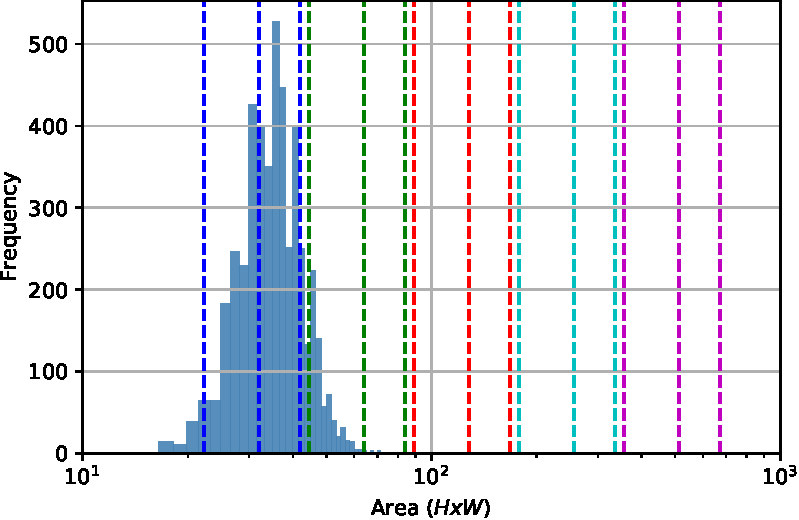
\includegraphics[width=0.45\textwidth]{figures/ch3/fig2_1.pdf}
    \label{fig2_1}
  }
  \subfigure[Validation dataset.]{
    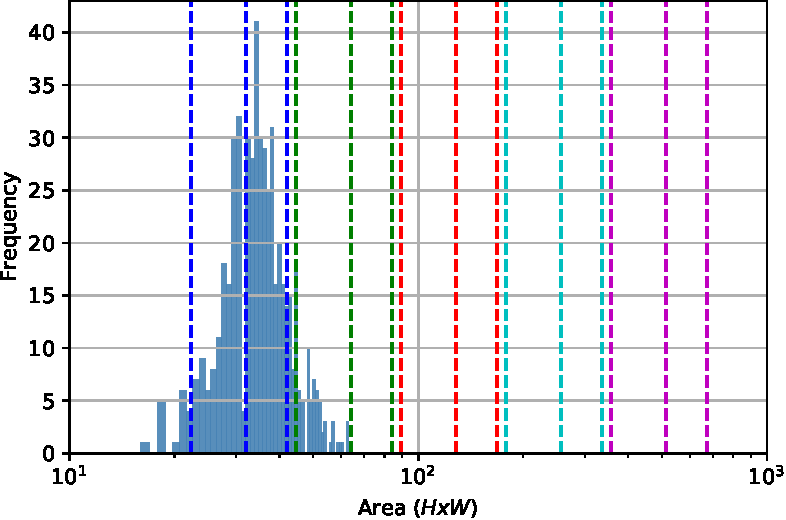
\includegraphics[width=0.45\textwidth]{figures/ch3/fig2_2.pdf}
    \label{fig2_2}
  }
  \caption{The annotation boxes' area distribution, along with the scaled optimised anchor boxes. It can be seen that the anchors of the last 3 layers are almost redundant.}
  \label{fig2}
\end{figure}

\subsection{Hyper-parameter Selection}
The IoU threshold to consider a detection as a true positive was set equal to $IoU_{th} = 0.2$ (as in \cite{bargoti2017deep} to perform valid comparisons). The confidence score for the proposed detections was set as $p(c_i) > 0.05$ and the $\text{NMS}_{th}$ was set equal to 0.3, as it found out to be the best after experimentation. To save computation time the maximum proposed detections allowed was set to be 100. 

Finally, concerning the loss function, tweaking $\alpha$ and $\gamma$ did not yield any difference in performance, so the default parameters $\alpha=0.25$ and $\gamma=2$ remained unchanged. A notable remark is that the loss function was found to be very unstable during training. The reason was that the normalisation parameters take values equal to the total number of the instances in the image. This behaviour is a result of the increased variance exhibited by the Fruit/Img., as can be seen in \tref{tab1}. To tackle this issue, the normalisation factor was modified, taking values from an exponential moving average of the total instances in the samples.
 
\section{Proposed Architectures}
RetinaNet network exploits the inherent multi-scale, pyramidal hierarchy of the backbone network making predictions in multiple scales. Deeper layers capture higher levels of abstraction, making coarser feature maps semantically stronger comparing to finer feature maps. Rougher feature maps are also useful for predicting bigger objects due to their receptive field. \fref{fig1} shows that detection from higher pyramidal levels might be redundant. 

The proposed architectures explore:
\begin{itemize}
 \item the depth impact of the backbone through the VGG11, VGG13, VGG16 and VGG19 architectures
 \item and the topology of the side network of RetinaNet, responsible for the detection part.
\end{itemize}

Inference time, network's number of parameters and the need in computational and memory resources can be further reduced through an optimised network, that achieves maximum performance at the same time.

\textbf{Architectures}
\begin{itemize}
 \item{\textbf{Original}:}\label{arch_1} 
The first architecture, original RetinaNet, uses 5 pyramidal levels (P3,P4,P5,P6,P7) for prediction. P3, P4 and P5, are obtained via lateral connections right after the corresponding VGG blocks (reduced in a fixed depth of $\times256$) and are semantically enhanced as shown in the right-left pathway in \fref{fig3}. P6 and P7 are obtained from single $3\times3$ strided convolutions after the last VGG convolutional block. Finally, a common predictor and box regressor makes predictions from each layer.

\begin{figure}[!htb]
  \centering
  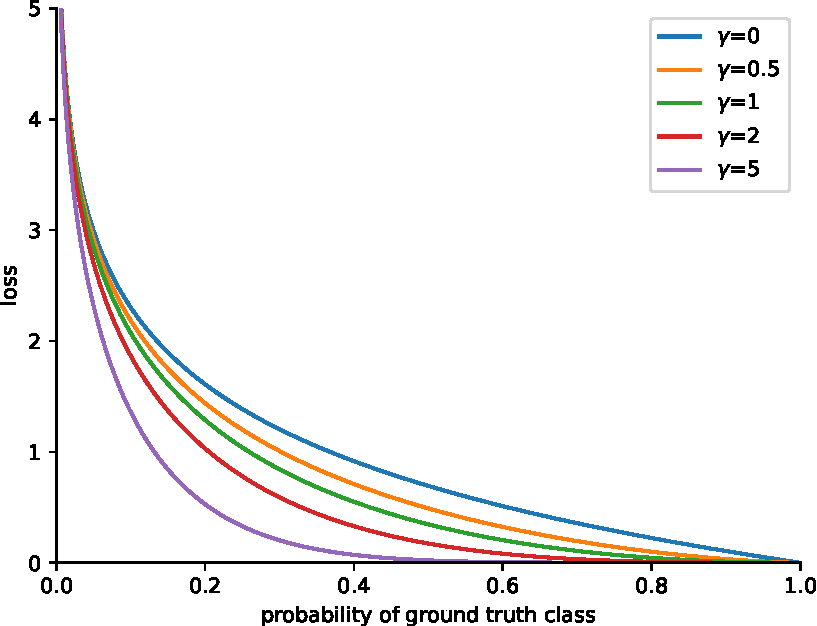
\includegraphics[width=0.5\textwidth]{figures/ch3/fig3.pdf}
  \caption{The original RetinaNet pipeline. No. of parameters: 8.7M (without VGG).}
  \label{fig3}
\end{figure} 

 \item{\textbf{$\text{P}_3\text{P}_4\text{P}_5$}:}\label{arch_2}
The second architecture follows the original RetinaNet structure, without utilising P6 and P7 at all. P3, P4, P5 still follows the upsampling-merging technique. The difference with the original architecture is that it is incapable of detecting objects ranging  between $200^2$ - $700^2$ pixels.

\begin{figure}[!htb]
  \centering
  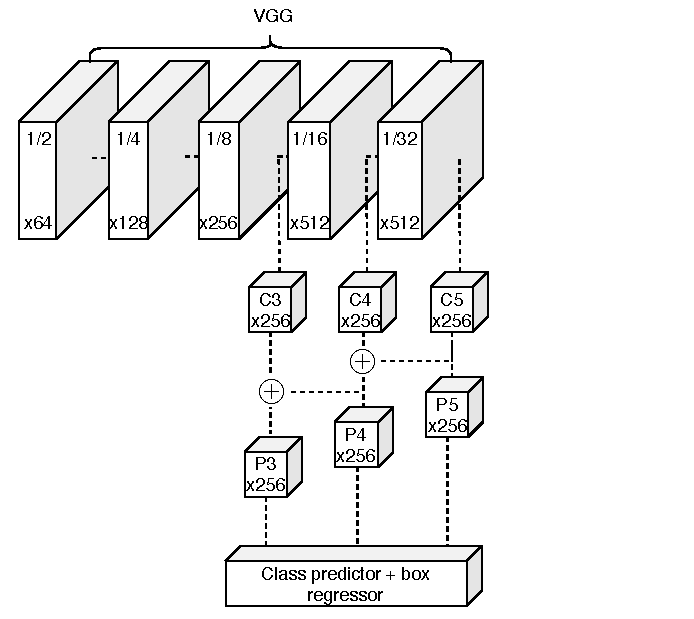
\includegraphics[width=0.5\textwidth]{figures/ch3/fig4.pdf}
  \caption{RetinaNet - $\text{P}_3\text{P}_4\text{P}_5$: A slightly different version of RetinaNet without using P6 and P7 . No. of parameters: 6.9M (without VGG).}
  \label{fig4}
\end{figure} 

 \item{\textbf{$\text{P}_\text{i}\text{Multi}$}:}\label{arch_3}
The next architecture is similar to the previous. However, instead of sharing common classification and regression heads, each $P_i$ has separate classifiers and regressors with unshared parameters. This architecture is much more computationally and memory expensive, however, the reasoning behind this deployment is to investigate if by attaching multiple classification and regression heads, there is any gain in performance.

\begin{figure}[!htb]
  \centering
  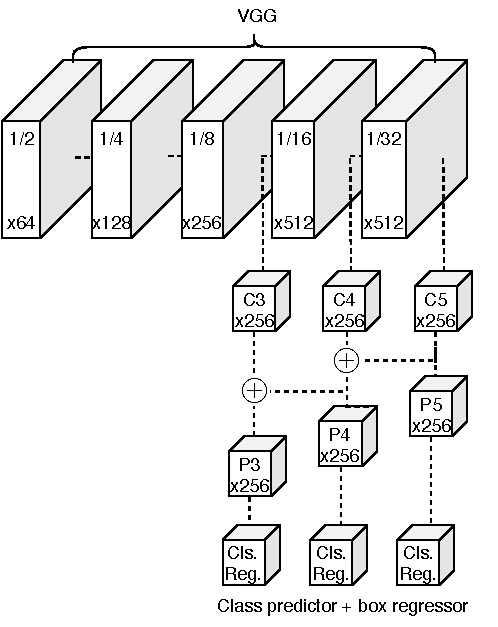
\includegraphics[width=0.5\textwidth]{figures/ch3/fig5.pdf}
  \caption{RetinaNet - $\text{P}_\text{i}\text{Multi}$: A modified Architecture - 2 with separate classification. and regression submodel. No. of parameters: 16.6M (without VGG).}
  \label{fig5}
\end{figure} 

 \item{\textbf{$\text{C}_\text{i}\text{Reduced}$}:} 
Finally, the last configuration is the lightest among all. It utilises only the reduced in depth feature maps obtained right after block 3, block4 and block 5 from VGG by attaching common classifier and box regressor heads. It is inspired by the SSD (\cite{liu2016ssd}), but is considerably lighter, as it skips the extra layers after block 5 of the VGG network.

\begin{figure}[!htb]
  \centering
  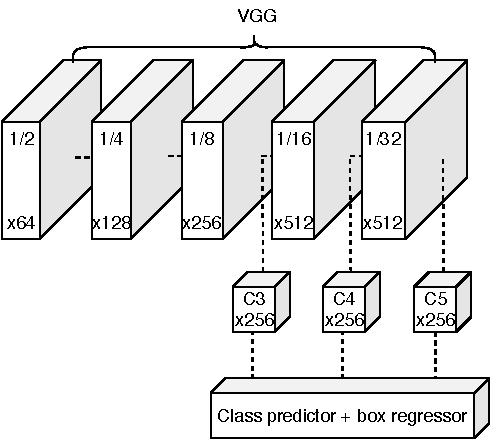
\includegraphics[width=0.5\textwidth]{figures/ch3/fig6.pdf}
  \caption{RetinaNet - $\text{C}_\text{i}\text{Reduced}$: The lightest architecture, inspired by the SSD, but more much shallower. No. of parameters: 5.1M (without VGG).}
  \label{fig6}
\end{figure} 

\end{itemize}


%% ----------------------------------------------------------------
%% Conclusion.tex
%% ---------------------------------------------------------------- 
\chapter{Conclusion and Future Work} \label{Chapter: Conclusion}
This thesis aimed to investigate the apple detection problem using the deep learning-based algorithm, RetinaNet. Previous works have repeatedly demonstrated the superiority of deep learning-based methods for agricultural purposes, especially in the field of fruit detection. The biggest advantage of deep learning is that it entirely dismissed feature engineering, which requires expertise from the domain knowledge; thus, it enabled the development of algorithms that apply in universal datasets instead of being crop-specific.

RetinaNet exploits the pyramidal feature hierarchy of the backbone network to build higher-level semantic maps. From each intermediate backbone layer, it obtains feature maps of different spatial sizes, each containing different levels of information. Combination of coarse feature maps rich in information with spatially larger semantically weak maps, results in finer maps, which contain large amounts of information. The resulting feature maps are five pyramidal levels of increasing resolution, each with high content in semantic information, thus enabling detection at multiple scales.

The hyper-parameter tuning is essential for the efficient optimisation of the pipeline. However, in the latest works in the field of fruit detection, hyper-parameter optimisation does not seem that have been analysed in-depth. In the present study, the right predefined anchor boxes' sizes have been efficiently configured through an evolution search algorithm, enabling easier regression. Furthermore, loss function has been modified to adopt more stable values in order to accelerate convergence. Moreover, an analysis between the dataset's annotation size distribution and the predictions' sizes from each pyramidal level of RetinaNet showed, that some layers might be redundant. This observation suggests that different and simpler architectures should be explored. In this way, the present thesis focused on the study of side-network's efficiency through four proposed alternative deployments.

Concerning the network's effectiveness, it was demonstrated that performance scales with the depth of the backbone network; however, that was not the case with the side-network. The lightweight RetinaNet - $\text{C}_\text{i}\text{Reduced}$ consistently performed better compared to more sophisticated architectures. These results suggest that this binary problem is not benefited neither by semantically enriching the feature maps nor by increasing side-network's complexity in a different way.

Surprisingly, an investigation of the performance-training size relationship revealed that even 10 samples are enough for adequate detection. Moreover, maximum performance was achieved by using only 200-500 samples, that is at least 2x times less than the original training set. In this way, growers would be relieved from labelling big datasets. This finding raises questions around the dataset, since it known that the performance of deep learning algorithms scales with the size of the training dataset.

In the last section, optimisation for peak detection demonstrated that, indeed, high resolutions yield better results, but with infinitesimal difference. However, upon increasing resolution the training and inference time increases as well. RetinaNet - $\text{C}_\text{i}\text{Reduced}$ (VGG16) reached its maximum performance with AP=\textbf{0.955} and F1=\textbf{0.908} using a resolution of $800\times1220$, outperforming the state-of-the-art (\cite{bargoti2017deep}). The same model trained on dataset's original resolution ($202\times308$), achieved an AP=\textbf{0.948} and an F1-score=\textbf{0.895} making detections at roughly \textbf{70} FPS, x1.5 times faster than the model of \cite{liang2018apple}. RetinaNet - $\text{C}_\text{i}\text{Reduced}$ is the lightest model with the smallest memory footprint among the rest; it has only 19.8M parameters coupled with VGG16, while VGG19 has 20M parameters itself. Furthermore, the model managed to maintain its first-rate performance even under the more strict $\text{IoU}_{th}$ of 0.5.

Concerning model's limitations, as shown in \sref{nms_threshold}, the detector suppresses detections with overlap $\text{IoU}\geq\text{NMS}_{th}$, as these predictions are registered as multiple detections (Figures \ref{ch6:fig4_2}, \ref{ch6:fig4_3} and \ref{ch5:fig6} demonstrate this behaviour). However, the severity of this problem depends on the context of the application that the framework may be implemented into. For instance, in the case of robotic harvesting it is not crucial, as after a fruit has been gathered, the algorithm can update the detected instances through a new image. On the contrary, in yield estimation applications the model will always undercount, leading in inaccurate results. Furthermore, acquiring data with monocular cameras make the model prone to double-counting, as the model does not identify the objects across frames. As a result, farmers should put extra effort into obtaining datasets with unique instances. Lastly, monocular RGB cameras are incapable of estimating depth; thus the model struggles to distinguish between foreground and background (\fref{ch6:fig3}) resulting in learning spurious rules, such as classifying relevant objects by their relative size.

The ACFR dataset consists of crops of images that span entire trees in an orchard block. The proposed technique can be commercialised through a robotic harvesting application from unmanned ground vehicles, as it allows accurate detections from images captured in relatively short distances. Future work, could involve the exploration of the algorithm's full potential in real-time detection, e.g. in the case of integrating the system on drones, flying between orchard rows. This can be studied through sequential images of entire trees without sub-sampling, in order to investigate if the state-of-the-art performance can be preserved on samples with smaller fruits. Integrating a tracking system on the main pipeline, such as the Hungarian Algorithm, can provide accurate yield mappings.

Finally, concerning the ACFR dataset, RetinaNet achieved similar performance with previous studies in apple detection, through the same dataset in terms of F1-score. In \sref{size_relation}, it was observed that state-of-the-art F1-score reached its peak already from the first 500 samples. This observation combined with several dubious truth annotations, as seen in \fref{ch6:fig4_2}, advocates the reexamination of the ACFR dataset in terms of more reliable ground truth annotations.


 \begin{figure}[!ht]
  \centering
  \subfigure[]{
    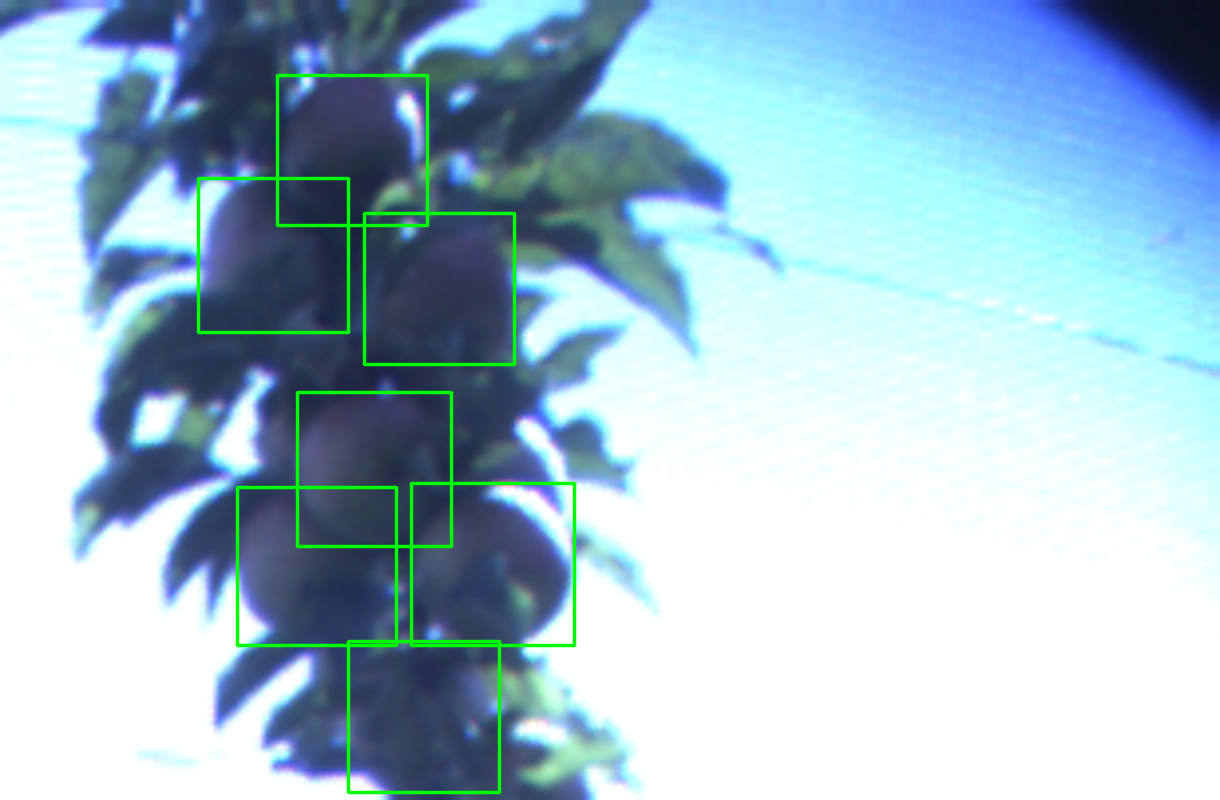
\includegraphics[width=0.31\textwidth]{figures/ch6/fig1_1.png}
    \label{ch6:fig1_1}
  }
  \subfigure[]{
    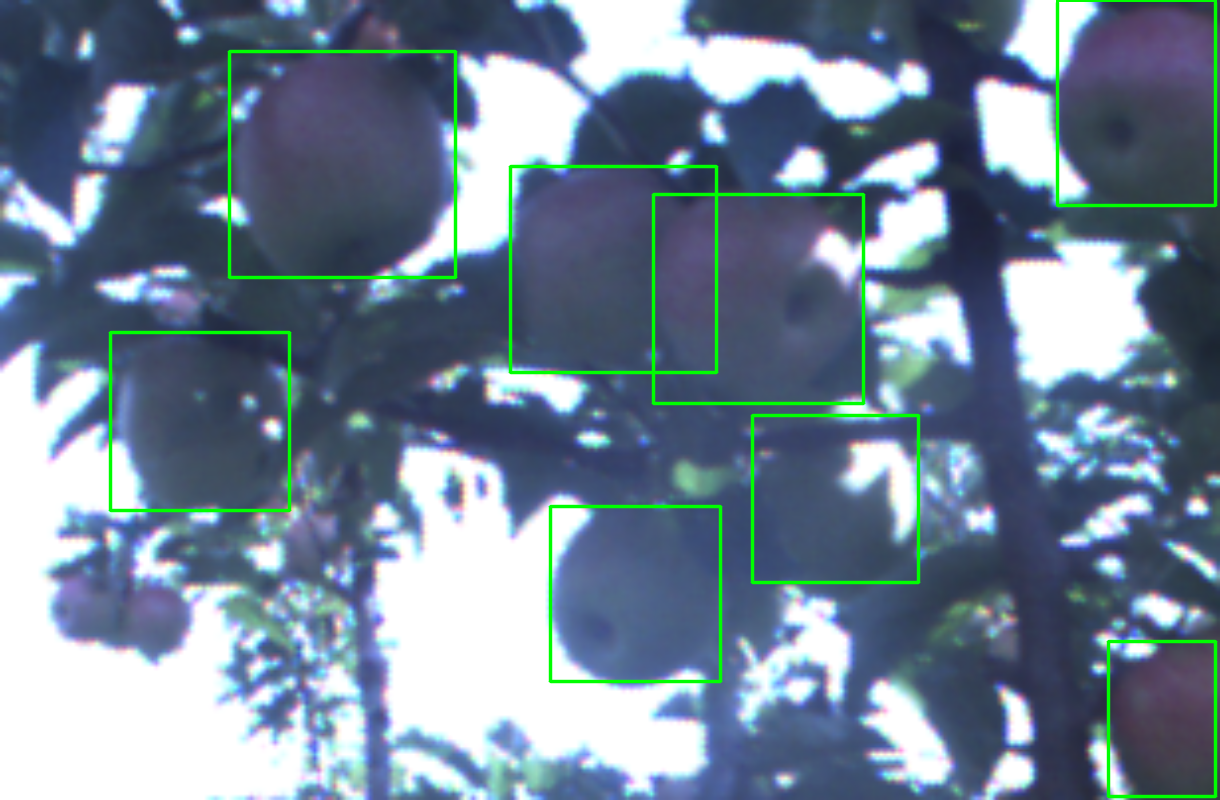
\includegraphics[width=0.31\textwidth]{figures/ch6/fig1_2.png}
    \label{ch6:fig1_2}
  }
  \subfigure[]{
    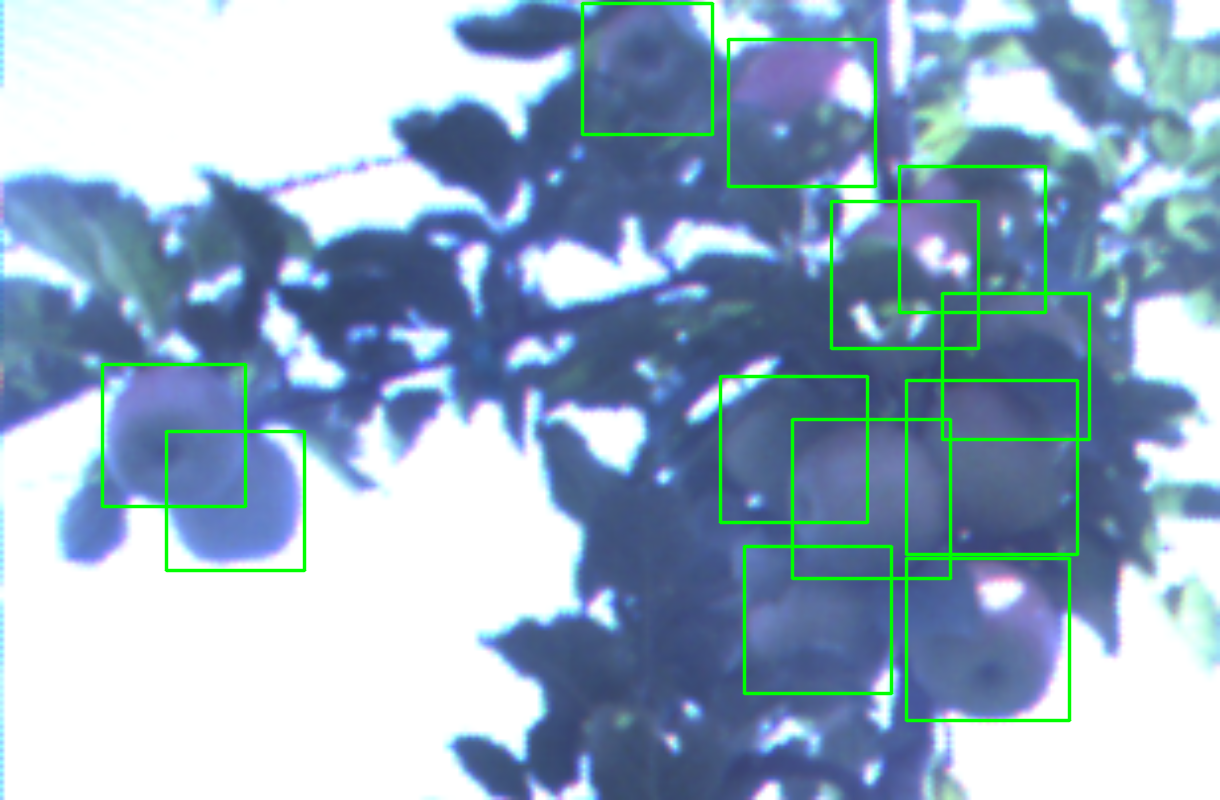
\includegraphics[width=0.31\textwidth]{figures/ch6/fig1_3.png}
    \label{ch6:fig1_3}
  }
  \caption{Cases of successful predictions: (a) in a tight fruit cluster, (b) between foreground and background fruits (bottom-left) and (c) in a fruit cluster with highly occluded instances. Green boxes represent true positive examples.}
  \label{ch6:fig1}

  \subfigure[]{
    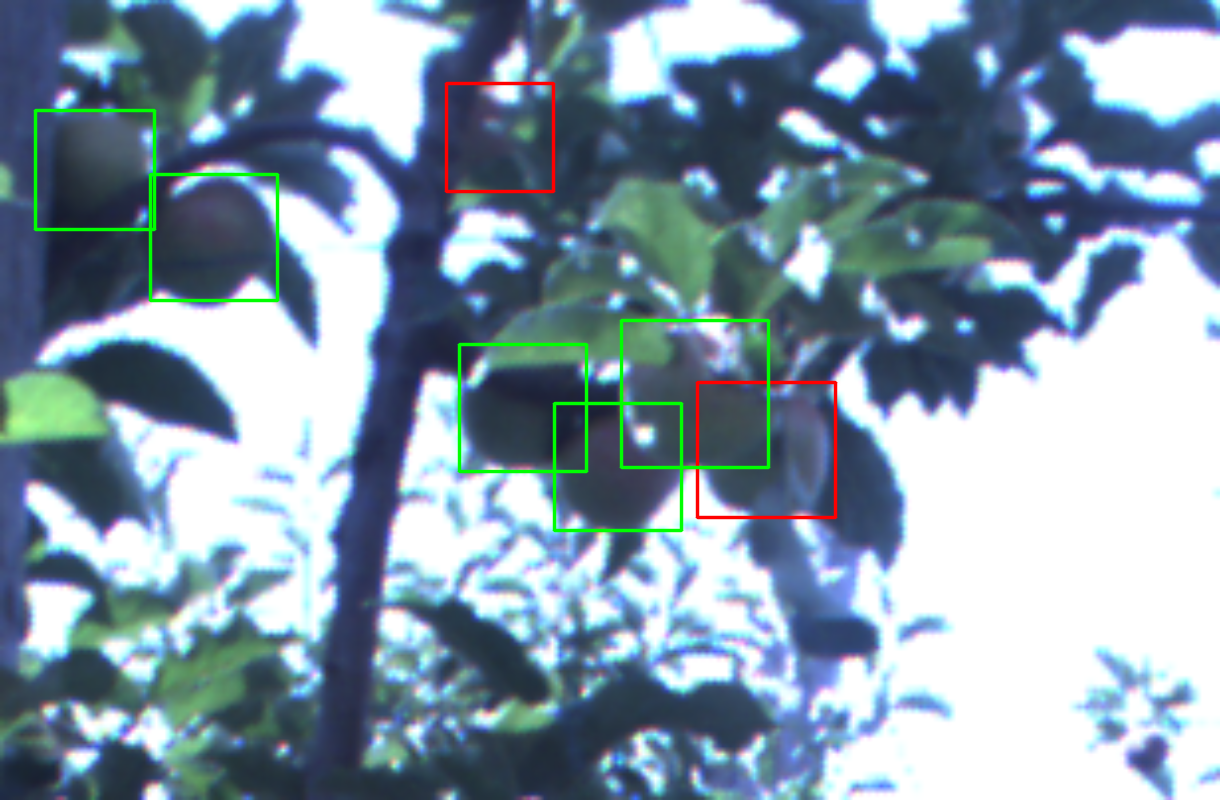
\includegraphics[width=0.31\textwidth]{figures/ch6/fig2_1.png}
    \label{ch6:fig2_1}
  }
  \subfigure[]{
    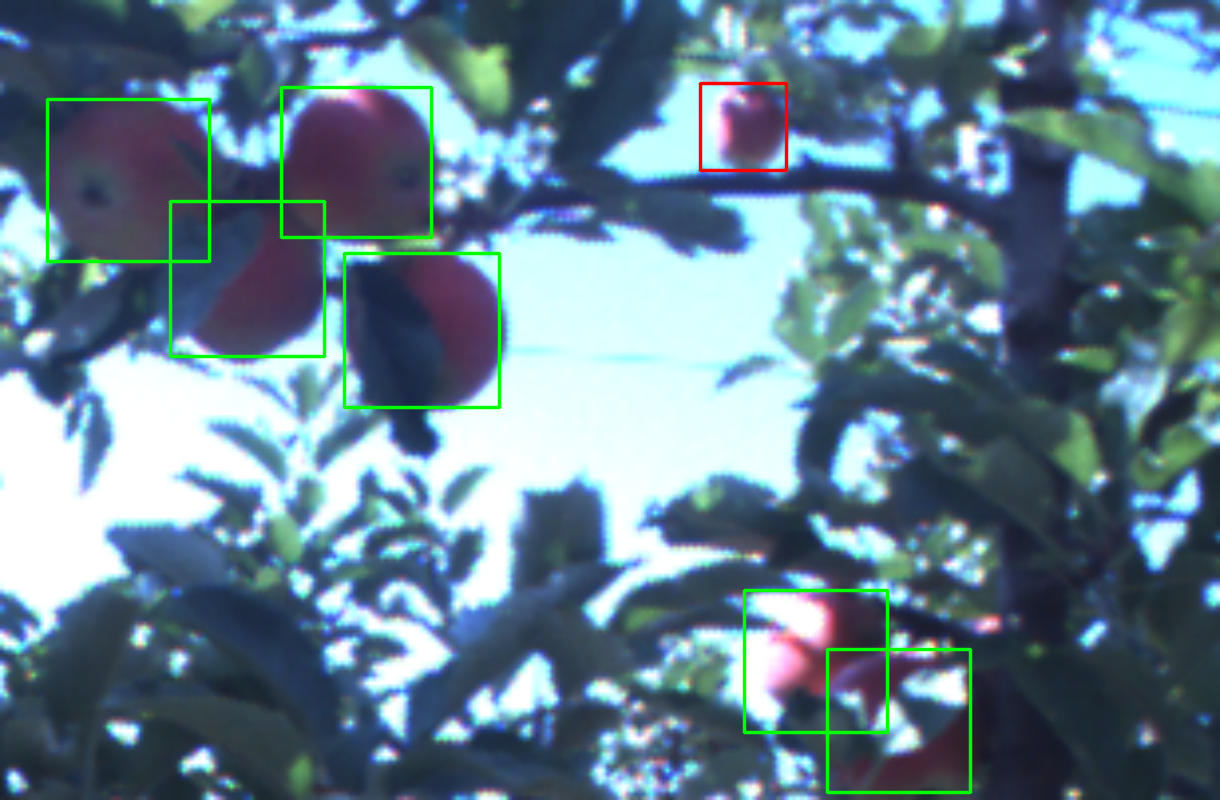
\includegraphics[width=0.31\textwidth]{figures/ch6/fig2_2.png}
    \label{ch6:fig2_2}
  }
  \subfigure[]{
    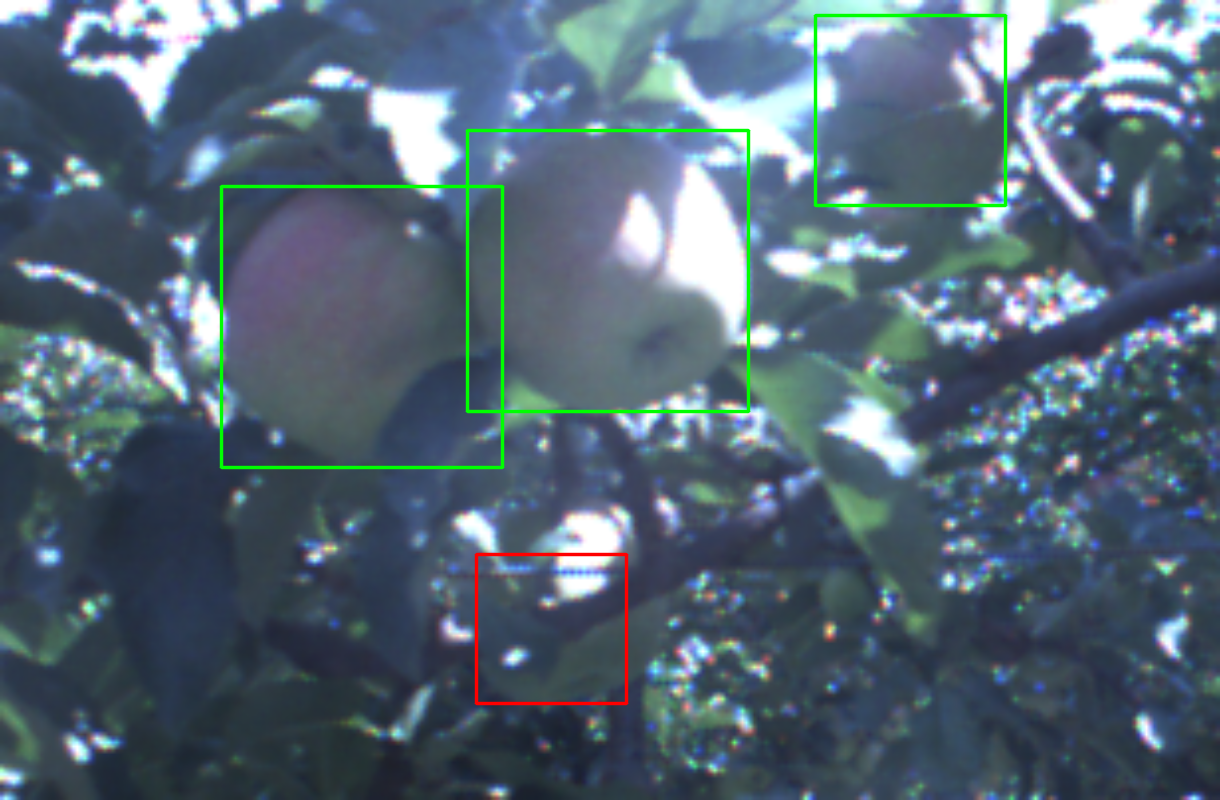
\includegraphics[width=0.31\textwidth]{figures/ch6/fig2_3.png}
    \label{ch6:fig2_3}
  }
  \caption{Error cases where apparently correct predictions are registered as false positives due to lack of annotation. Green and red boxes represent true and false positives respectively.}
  \label{ch6:fig2}

  \subfigure[]{
    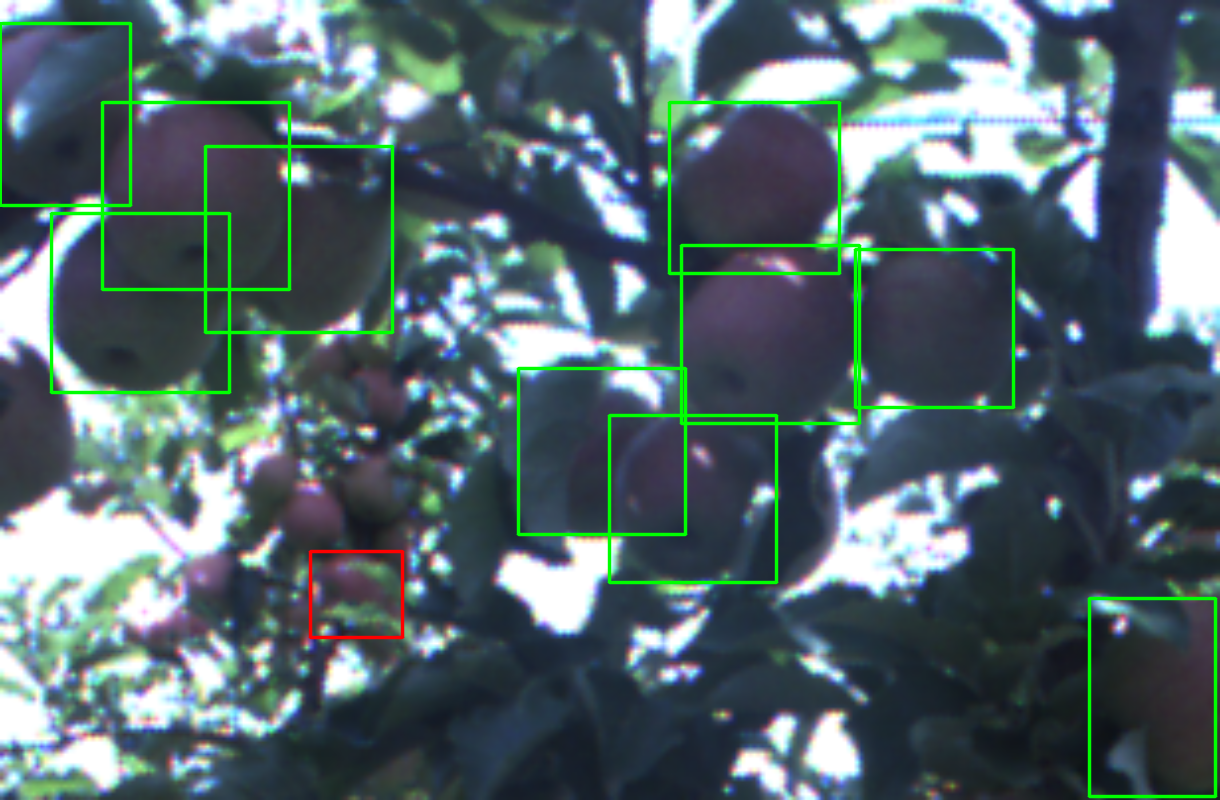
\includegraphics[width=0.31\textwidth]{figures/ch6/fig3_1.png}
    \label{ch6:fig3_1}
  }
  \subfigure[]{
    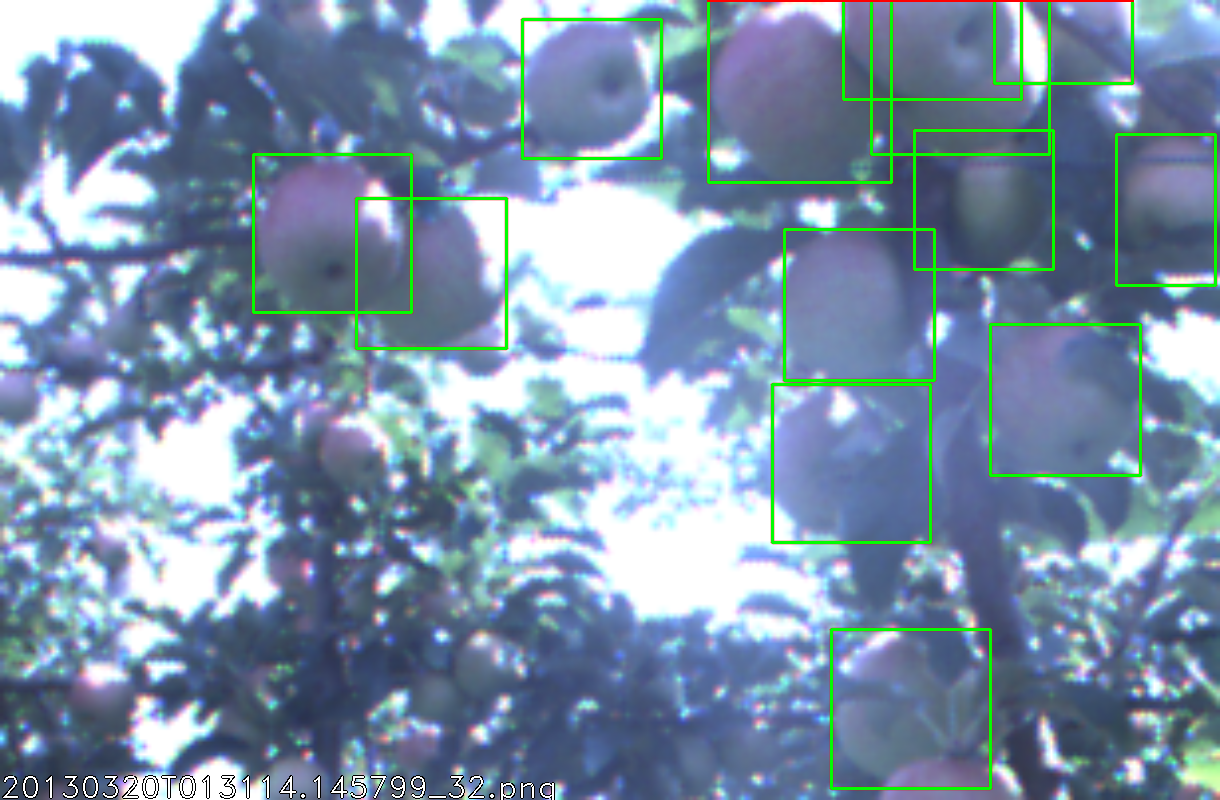
\includegraphics[width=0.31\textwidth]{figures/ch6/fig3_2.png}
    \label{ch6:fig3_2}
  }
  \subfigure[]{
    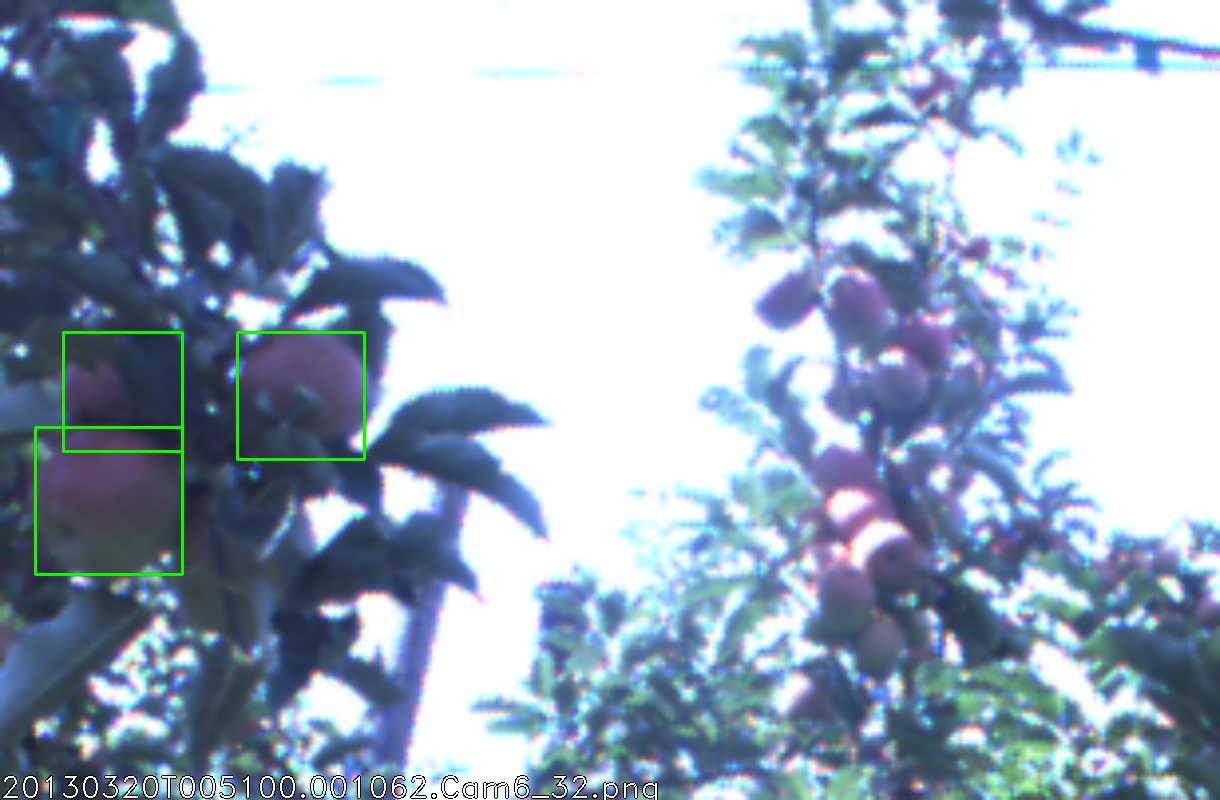
\includegraphics[width=0.31\textwidth]{figures/ch6/fig3_3.png}
    \label{ch6:fig3_3}
  }
  \caption{Some correctly classified hard examples in the training dataset; however, it is disputed if classification to foreground and background was done by fruits' relative size. The model encounters difficulties identifying relevant samples between foreground and background. If the model associates foreground with the relative fruit size, this misleading rule indicates overfitting, as it does not apply in general. Green and red boxes represent true and false positives respectively.}
  \label{ch6:fig3}

  \subfigure[]{
    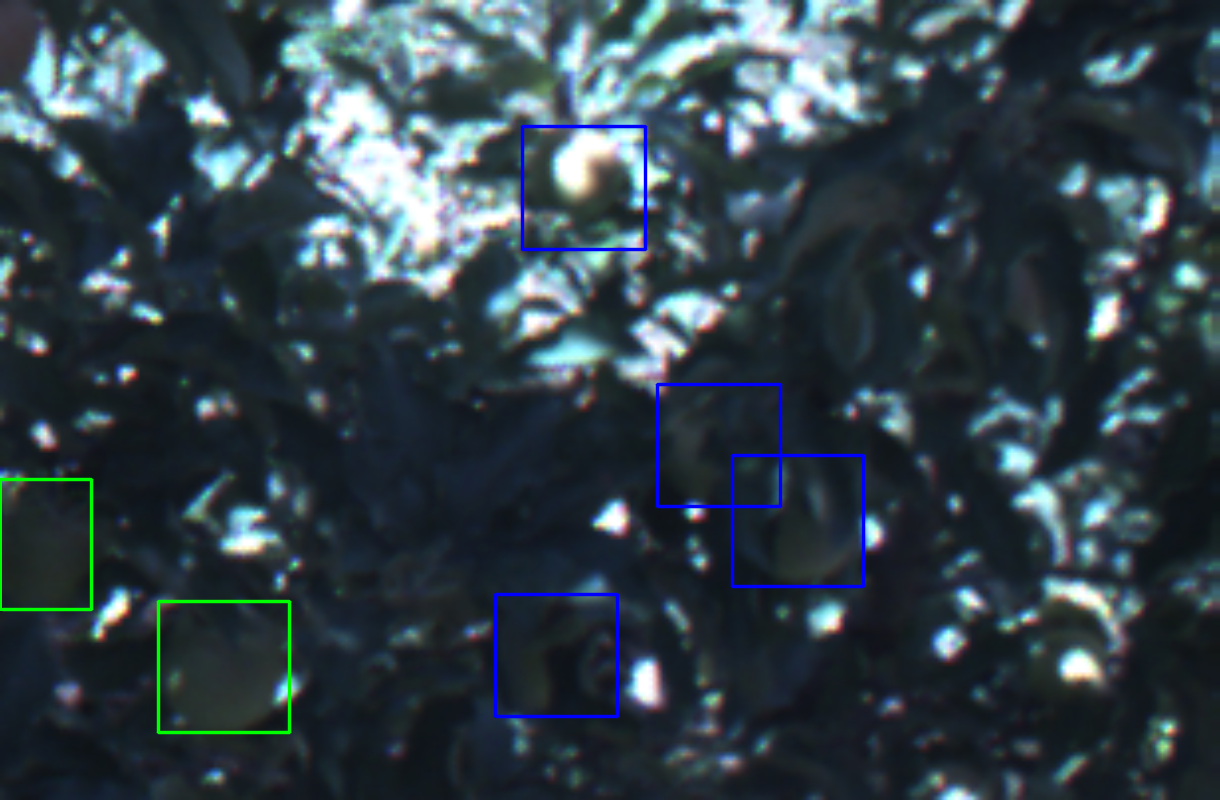
\includegraphics[width=0.31\textwidth]{figures/ch6/fig4_1.png}
    \label{ch6:fig4_1}
  }
  \subfigure[]{
    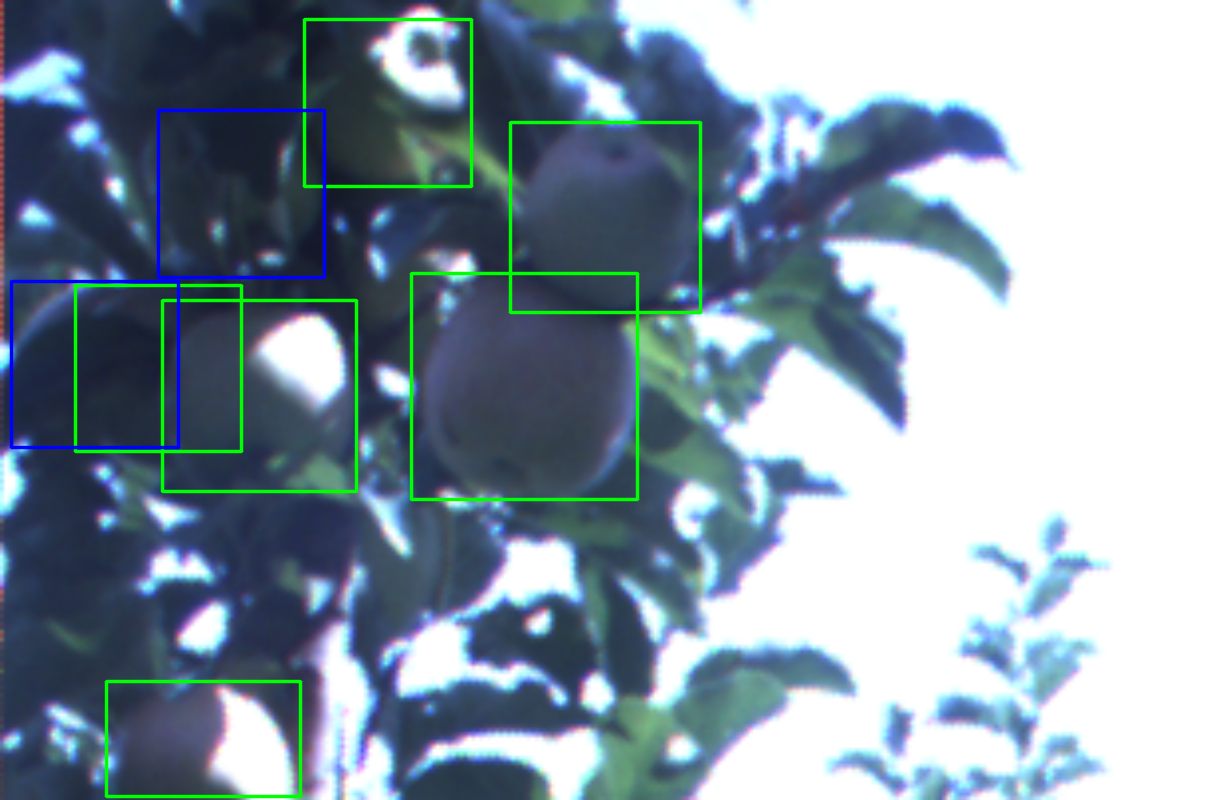
\includegraphics[width=0.31\textwidth]{figures/ch6/fig4_2.png}
    \label{ch6:fig4_2}
  }
  \subfigure[]{
    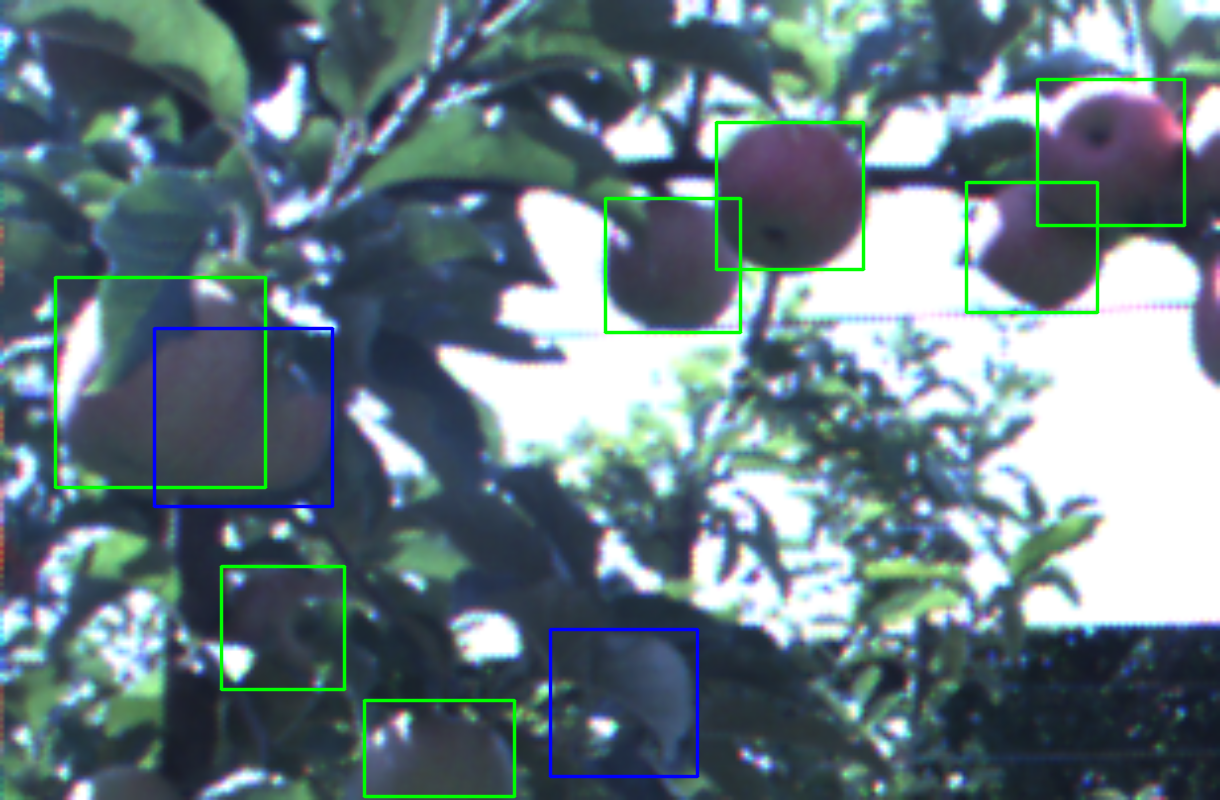
\includegraphics[width=0.31\textwidth]{figures/ch6/fig4_3.png}
    \label{ch6:fig4_3}
  }
  \caption{Interesting false negative predictions from the testing dataset. Errors due to: (a) illumination conditions, (b-c) dubious ground truths. In (b-c), it can be seen that occluded instances with $\text{IoU} \geq \text{NMS}_{th}$ are suppressed to avoid multiple detections of the same object. Green and blue boxes represent true positives and false negatives respectively.}
  \label{ch6:fig4}
\end{figure}



\appendix
%% ----------------------------------------------------------------
%% AppendixA.tex
%% ---------------------------------------------------------------- 
\chapter{Package versions} \label{pack_versions}
The following gets in the way of the text....

\backmatter
\bibliographystyle{ecs}
\bibliography{ECS}
\end{document}
%% ----------------------------------------------------------------
